% ============================================================================
%  Active-Ledger: Trust-Gated Diffusion and Behavioural Contribution Scoring
%  for Adversarially Robust Federated ECG Arrhythmia Classification
%
%  Target venue: ESORICS (single-blind)
%  Template: Springer LNCS (llncs.cls)
%  Authors: disclosed (place real names + affiliations before submission)
% ============================================================================

\documentclass[runningheads]{llncs}

% -- Packages (minimal, LNCS-safe) -------------------------------------------
\usepackage[T1]{fontenc}
\usepackage{amsmath,amssymb}
\usepackage{graphicx}
\usepackage{booktabs}
\usepackage{array}
\usepackage{url}
\usepackage{xspace}
\usepackage{placeins}   % \FloatBarrier: keep figures near their discussion
% Architecture diagram (TikZ)
\usepackage{tikz}
\usetikzlibrary{arrows.meta,positioning,calc}
% hyperref last so \ref{fig:*} references become clickable links in the PDF
\usepackage[colorlinks=false,linktoc=all,linktocpage,hidelinks]{hyperref}

% Short names for defences so prose stays light
\newcommand{\fedavg}{\textsc{FedAvg}\xspace}
\newcommand{\krum}{\textsc{Krum}\xspace}
\newcommand{\mkrum}{\textsc{Multi-Krum}\xspace}
\newcommand{\median}{\textsc{Median}\xspace}
\newcommand{\tmean}{\textsc{Trimmed-Mean}\xspace}
\newcommand{\bulyan}{\textsc{Bulyan}\xspace}
\newcommand{\poc}{\textsc{PoC}\xspace}
\newcommand{\actledger}{\textsc{Active-Ledger}\xspace}
\newcommand{\tgldm}{Trust-Gated LDM\xspace}
\newcommand{\bldm}{Blind LDM\xspace}
\newcommand{\apbf}{APB-F1\xspace}

% ----------------------------------------------------------------------------
\begin{document}

\title{Active-Ledger: Trust-Gated Diffusion and
Behavioural Contribution Scoring for Adversarially Robust
Federated ECG Arrhythmia Classification}
\titlerunning{Active-Ledger: Trust-Gated Diffusion for Robust Federated ECG}

\author{ Muhammad Maaz Siddiqui\and
Muhammad Ibrahim Farid\and
Muhammad Ibrahim Iqbal \and
Faisal Iradat}
\authorrunning{Siddiqui et al.}

\institute{Institute of Business Administration, Karachi, Pakistan\\
\email{\{m.farid.27098,m.siddiqui.27070,m.iqbal.27085,firadat\}@khi.iba.edu.pk}}

\maketitle

% ============================================================================
\begin{abstract}
Federated learning (FL) is a natural fit for clinical electrocardiography:
hospital data never leaves the hospital, while the shared model still
benefits from every site. A clinical deployment has to survive two
problems at once. Hospital data is highly non-independent and identically
distributed (non-IID), and adversaries that
get a foothold will preferentially target the rare, clinically dangerous
classes. This paper introduces \actledger, a blockchain-orchestrated
FL system whose defence is behavioural rather than geometric and
which also closes a second attack surface that classical robust
aggregation never looks at: the augmentation channel that opens when
a diffusion generator is added to repair rare-class deficit. The
Proof-of-Contribution score proposed here is a simple, on-chain,
history-based contribution score; it is not a cryptographic proof.
It is paired with a trust-gated class-conditional 1D latent diffusion
model (LDM) generator, and the ledger records every aggregation and
every generation as an immutable event. \actledger is evaluated on
MIT-BIH arrhythmia classification under three attacks (Gaussian weight
poisoning, static label-flip, and a sleeper backdoor-critical-layer flip
that activates mid-training), against six baselines (\fedavg, \krum,
\mkrum, \median, \tmean, \bulyan). Across all three attacks, \poc is the
only defence that keeps atrial-premature-beat (APB, Class~3) F1 above
the $0.75$ deployability line. Adding trust-gated diffusion then pushes
APB-F1 to $0.879$ under the sleeper attack, beating an un-gated
\mkrum\,+\,\bldm baseline on both APB-F1 and final-round backdoor
success rate.

\keywords{Federated learning \and Blockchain \and Byzantine robustness
\and Backdoor attacks \and Diffusion models \and Clinical IoT.}
\end{abstract}

% ============================================================================
\section{Introduction}
\label{sec:intro}

Federated learning ~\cite{mcmahan2017fedavg,kairouz2021advances}
has become the default recipe whenever training data is locked up at
the edge, and clinical electrocardiography (ECG) fits the recipe
cleanly. The MIT-BIH Arrhythmia Database~\cite{moody2001mitbih},
preprocessed under AAMI EC57~\cite{aami1998ec57}, is the benchmark
that almost every arrhythmia paper returns to. MIT-BIH is also a
textbook case of class imbalance, and its rare classes are the ones
that matter clinically. An atrial premature beat (APB, Class~3 in
the AAMI mapping) is outnumbered by normal sinus rhythm roughly
twenty-seven to one; yet missing an APB delays atrial-fibrillation
work-up, and a false positive triggers a consult that did not need
to happen. Any FL system intended for deployment in this setting has
to hold the rare class together while it trains on very different
hospital distributions.

This is hard even without adversaries. Under non-IID FL, an honest
hospital's gradient often looks different from the crowd for
perfectly innocent reasons: many APB cases that week, mostly elderly
patients, or a particular equipment vendor. Classical Byzantine-robust
aggregation rules -- \krum~\cite{blanchard2017krum}, \mkrum,
coordinate-wise \median and \tmean~\cite{yin2018byzantine}, and
\bulyan~\cite{elmhamdi2018bulyan} -- all defend by per-round geometry:
they filter clients whose weight vectors sit far from the consensus
of that round. The same filter also punishes honest non-IID outliers,
and Fang et al.~\cite{fang2020local} showed that these rules can be
defeated by attacks explicitly crafted to sit inside the geometric
envelope. The backdoor-FL line~\cite{bagdasaryan2020how,foroughi2026lsa} has since confirmed that the
strongest attacks are stealthy and time-varying: a Byzantine client
can accumulate a good-citizen history in early rounds and only switch
to flipping labels once the global model has stabilised. There is no
geometric anomaly for a per-round rule to catch in the early rounds.

There is also a second attack surface that the Byzantine-FL
literature rarely addresses. If the federation uses a diffusion
generator~\cite{ho2020ddpm,rombach2022ldm} to patch up rare-class
deficit -- a natural choice for medical data -- a malicious client
can request synthetic samples of a minority class while passing a
flipped label. A class-conditional generator will produce samples
from the wrong manifold, and those samples then get stamped with the
attacker-chosen label during local training. This paper refers to the
mechanism as the augmentation stealth channel. It lives upstream of the aggregator;
no robust aggregation rule can close it, because by the time the
aggregator sees anything, the poison is already baked into the
training data.

\medskip
\noindent
\textbf{Contributions.} Both contributions revolve around the same
idea: an immutable behavioural history is enough to close problems
that per-round geometry cannot.
\begin{itemize}
\item \textbf{Rare-class integrity under attack.} A simple
behavioural score -- the exponential moving average of a client's
on-chain validation accuracy, multiplied by its participation
fraction -- keeps APB-F1 above $0.75$ under three qualitatively
different attacks: Gaussian weight poisoning, static label-flip, and
a round-$15$ sleeper label-flip inspired by the backdoor-critical-layer
work of Zhuang et al.~\cite{zhuang2024bclayers} and Foroughi et
al.~\cite{foroughi2026lsa}. Every baseline considered in this study
(\fedavg, \krum, \mkrum, \median, \tmean, \bulyan) falls below
$0.75$ on APB-F1 in at least one of the three regimes.
\item \textbf{Accountable augmentation.} Gating every synthetic-data
request with the same behavioural score, and writing every
aggregation and generation event to a smart contract, closes the
augmentation stealth channel. Against \mkrum combined with un-gated
diffusion -- a strong non-ledger baseline -- trust-gating raises
final APB-F1 from $0.857$ to $0.879$ and lowers the final-round
backdoor success rate.
\end{itemize}

PoC is not a consensus protocol and not a cryptographic proof;
it is a scalar contribution score. The ledger's only job in this
paper is to make the behavioural history, and every decision taken on
top of it, tamper-evident, so that the history cannot be rewritten and
post-hoc forensic inspection is possible. Section~\ref{sec:related}
places \actledger among existing contribution-aware and
committee-based blockchain-FL. Sections~\ref{sec:system}
and~\ref{sec:threat} describe the system and the attacks.
Section~\ref{sec:methods} specifies the defences and the two
augmentation policies. Section~\ref{sec:setup} gives the experimental
setup and Section~\ref{sec:results} presents the evaluation.
Section~\ref{sec:discussion} discusses limitations and
Section~\ref{sec:conclusion} concludes.

% ============================================================================
\section{Background and Related Work}
\label{sec:related}

\paragraph{Byzantine-robust aggregation.}
FL was introduced by McMahan et al.~\cite{mcmahan2017fedavg} together
with the \fedavg algorithm, which aggregates client updates by a
sample-weighted mean. The Byzantine-FL line began with
\krum~\cite{blanchard2017krum}: at every round the server selects the
single client whose summed squared distance to its closest neighbours
is minimal. \mkrum extends \krum by averaging several lowest-scored
clients. Yin et al.~\cite{yin2018byzantine} analysed coordinate-wise
\median and \tmean and proved order-optimal statistical rates, and
El Mhamdi et al.~\cite{elmhamdi2018bulyan} composed these ideas into
\bulyan. Fang et al.~\cite{fang2020local} later demonstrated that all
four can be fooled by local-model poisoning attacks explicitly
crafted to survive geometric filtering -- which is what motivates
looking beyond single-round geometry.

\paragraph{Backdoor federated learning.}
Bagdasaryan et al.~\cite{bagdasaryan2020how} showed that a
constrain-and-scale model-replacement attack can inject a backdoor
into the federated model while preserving its main-task accuracy.
Zhuang et al.~\cite{zhuang2024bclayers} observed that a small subset
of backdoor-critical layers carries almost all backdoor capacity, so
attacking only those layers bypasses seven contemporary defences with
just ten percent malicious clients. Foroughi et
al.~\cite{foroughi2026lsa} extended this with Layer Smoothing Attack,
in which the critical layers are blended into a distribution
indistinguishable from honest updates. The sleeper attack in
Section~\ref{sec:threat} operationalises the same core idea: a
time-switching attacker that behaves honestly until the global model
has stabilised, then flips labels. This is the worst case for
per-round geometric defences, because there is no geometric anomaly
in the early rounds that they could learn to filter.

\paragraph{Generative augmentation.}
Denoising Diffusion Probabilistic Models~\cite{ho2020ddpm} and Latent
Diffusion Models~\cite{rombach2022ldm} are the modern default for
class-conditional generation. Applying them to 1D ECG waveforms with
channel-concatenation conditioning is straightforward and has become
a standard tool for rare-class augmentation. The security literature
has not yet studied what happens when the generator is shared across
a federation with potentially Byzantine clients.

\paragraph{Blockchain-orchestrated and contribution-aware FL.}
Kim et al.'s BlockFL~\cite{kim2020blockfl} was among the first
designs to use a blockchain to exchange and verify local FL updates
without a central server. Subsequent work moved from passive logging
to contribution-aware participation: Kang et al.'s reputation-based
worker selection~\cite{kang2019incentive,kang2020reliable} maintains
a multi-weight subjective-logic reputation on a consortium blockchain
and uses it to decide which workers may join a round; recent
surveys~\cite{li2021bcflsurvey} cover the broader landscape of
committee-based coordination, incentives, and reputation management.
\actledger differs on three specific points. The contribution score
is kept deliberately minimal -- an exponential moving average of
on-chain validation accuracies with a participation fraction -- and
is framed explicitly as a score, not a consensus protocol. The same
score is used to gate augmentation requests, not just aggregation,
which is the new defensive use of the ledger. And the score is
evaluated under three attack models specifically chosen to expose the
limits of per-round geometry. The aim is not to compete with
reputation-FL on identity management, but to show that a minimal
history-based score, exposed on-chain so that selection and
augmentation decisions become accountable, is enough to close a class
of attacks that robust aggregators miss.

\paragraph{Clinical ECG federated learning.}
Brisimi et al.~\cite{brisimi2018ehr} is an early demonstration of
federated predictive modelling on electronic health records, and
later work applies FL to MIT-BIH and 12-lead
ECG~\cite{jimenez2024ecg}. These works largely assume an
honest-but-curious threat model, and they do not jointly consider
rare-class integrity and attacker participation in the augmentation
pipeline -- the gap \actledger addresses.

% ============================================================================
\section{System Model}
\label{sec:system}

\subsection{Participants and data partitioning}
The setting is a cross-silo FL deployment with ten participating
hospitals or ECG-cohort silos. Two are Byzantine; the remaining
eight behave honestly. Each honest client holds a locally stored subset of
MIT-BIH, partitioned by a Dirichlet distribution of concentration
$0.5$, which is the standard non-IID stress setting in the FL
literature. Some silos see mostly Normal beats; others see much
higher minority-class density.

The classifier is a compact CNN--LSTM that ingests a 360-sample
single-channel ECG window and returns one of five AAMI-standard
labels: Normal, left and right bundle branch block (LBBB and RBBB),
atrial premature beat (APB), and premature ventricular contraction
(PVC). The AAMI mapping and window length are both from
EC57~\cite{aami1998ec57}. Training runs for forty global rounds;
each round every participating client performs three local epochs of
Adam with learning rate $10^{-3}$ and batch size $128$. The local
cross-entropy loss uses clamped inverse-frequency class weights
(floor $0.3$, ceiling $10$), a standard imbalance handler applied
uniformly across every cell of the experimental grid so that class
imbalance is not a confound when defences are compared against each
other.

\subsection{What goes on-chain}
The FL server is paired with a smart contract deployed on a local
Ganache v7 Ethereum chain. The contract does not do any training --
it only logs what happened, through five event types. When a client
finishes local training the server writes an \texttt{UpdateLogged}
event with the client identifier, the round index, a hash of the
uploaded weights, and the locally reported validation accuracy.
When aggregation completes the server writes a
\texttt{RoundCompleted} event with a hash of the aggregated global
model. The synthetic-data pipeline uses three more event types:
\texttt{SyntheticRequested} when a client asks for help on a
deficient class, \texttt{SyntheticApproved} when the approval daemon
accepts the request, and \texttt{SyntheticGenerated} after the
generator has produced the samples. Because these receipts are
hash-chained, a later reviewer can reconstruct every decision the
server took about every client. All contract calls are wrapped in
defensive handlers so that a transient chain failure (for example a
Ganache nonce error) does not crash the round; the affected client
is given a neutral contribution score for that round and training
continues.

\subsection{Proof-of-Contribution score}
\label{subsec:poc}
The Proof-of-Contribution score turns the on-chain history into a
single number per client per round. For client $i$ at round $r$ it
is defined as
\begin{equation}
\mathrm{PoC}(i, r) \;=\;
\mathrm{EMA}_{\gamma}\!\left(\{\mathrm{acc}_{i, r'}\}_{r' \le r}\right)
\;\times\;
\frac{\lvert\mathcal{H}_i(r)\rvert}{r}.
\label{eq:poc}
\end{equation}
The first factor is an exponential moving average of the client's
validation accuracy up to round $r$, with smoothing constant
$\gamma = 0.7$ so that the average weights recent rounds more
heavily than older ones; a client that has just started to
misbehave sees its score drop within a handful of rounds. The
accuracy itself is evaluated against a small, fully anonymised
public proxy subset of the open-access MIT-BIH record set that the
orchestrator keeps purely as a benchmark; no private per-site data
ever leaves the client, so the score is computable without breaking
FL data-sovereignty. The second factor is the participation fraction
-- the fraction of rounds in which the client has a valid
\texttt{UpdateLogged} entry -- so that clients who skip rounds or
whose update never landed on-chain are penalised. The whole product
is clamped to the open interval $(10^{-6}, 1-10^{-6})$ to avoid
numerical edge cases.

PoC is used in exactly two places. The server ranks all clients by
their PoC score and forms the next global model as a
sample-size-weighted average of the top seven; and whenever a client
submits an on-chain synthetic-data request, the server approves it
only if the requester's PoC is at least $0.4$ (the trust threshold).
This second use is what the augmentation attack in
Section~\ref{sec:threat} targets and is the new defensive role of
the ledger in \actledger.

\subsection{Architecture overview}
The aggregation flow and the augmentation flow share the same score
and the same ledger; Fig.~\ref{fig:architecture} shows the two flows
together. In the aggregation flow the server collects local updates,
ranks clients by PoC, performs a weighted top-seven average, and
emits \texttt{UpdateLogged} and \texttt{RoundCompleted} receipts
along the way. In the augmentation flow a client that detects
rare-class deficit (fewer than $\max(50, 15\%)$ samples of some
class, whichever is larger) files an on-chain request; the approval
daemon checks the requester's PoC against the $0.4$ threshold, and
if it passes, invokes the class-conditional 1D-UNet latent diffusion
generator~\cite{ho2020ddpm,rombach2022ldm}, which returns $500$
synthetic samples of the requested class. A
\texttt{SyntheticGenerated} receipt is then written so the whole
chain of approval and generation is auditable.

\begin{figure}[!htbp]
\centering
\resizebox{1\linewidth}{!}{%
  % Standalone TikZ figure body for Fig.~\ref{fig:architecture}.
% Include from the main paper via: % Standalone TikZ figure body for Fig.~\ref{fig:architecture}.
% Include from the main paper via: % Standalone TikZ figure body for Fig.~\ref{fig:architecture}.
% Include from the main paper via: \input{figures_phase3/fig_architecture_tikz.tex}
%
% Design goals:
% - LNCS margin-safe (wrapped in \resizebox{...}{!}{...} by the caller)
% - Uncluttered: two horizontal flows (aggregation on top, augmentation below)
% - Close in structure to the provided reference diagram, but with clearer spacing
%
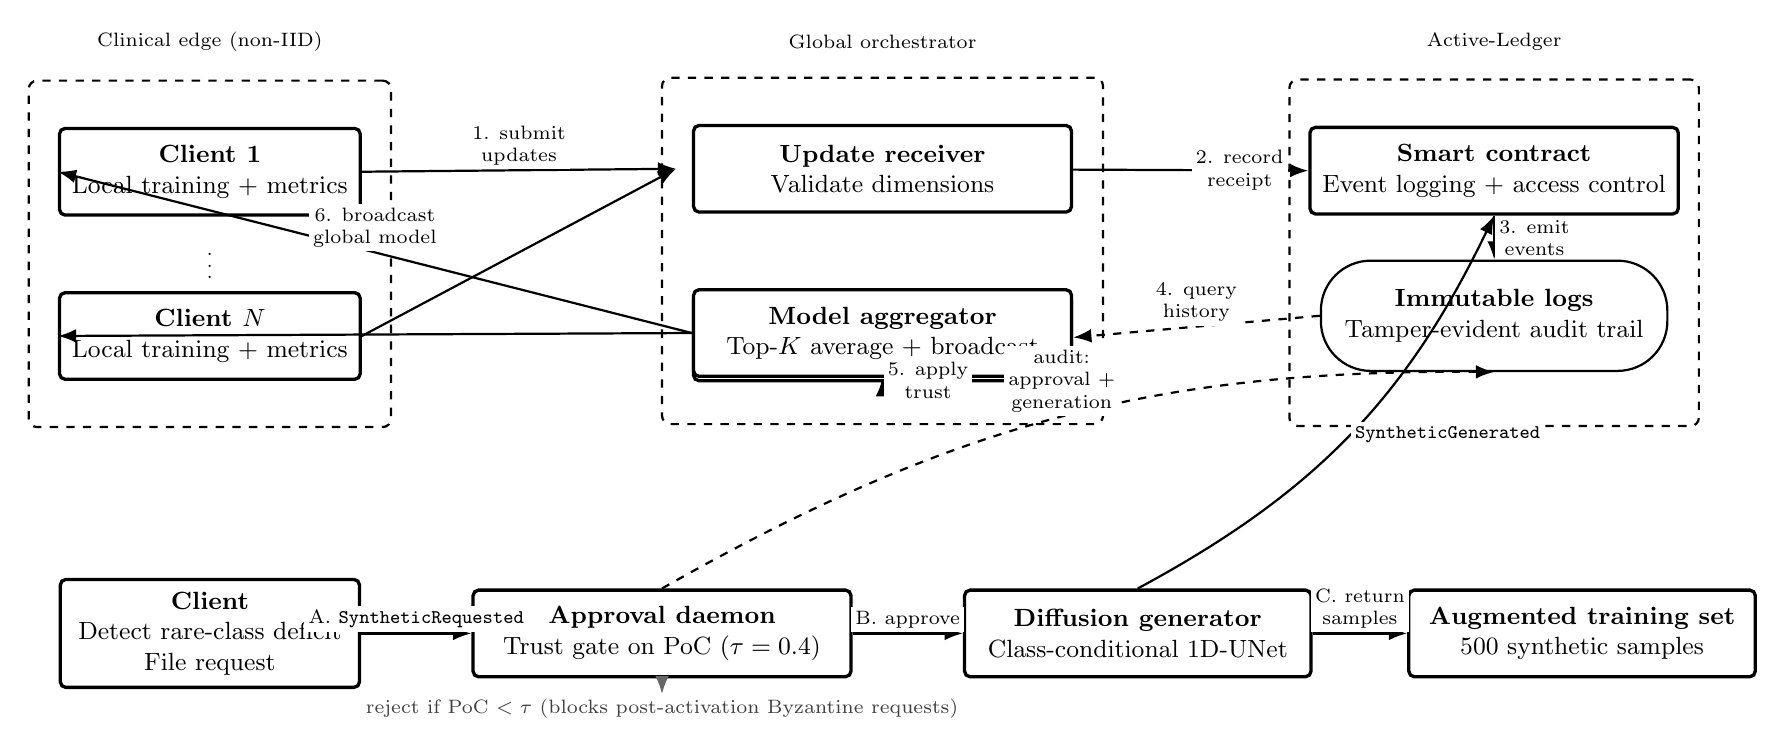
\begin{tikzpicture}[
  font=\small,
  node distance=7mm and 10mm,
  >=Latex,
  box/.style={draw, rounded corners=2pt, very thick, inner sep=4.5pt, align=center, fill=white},
  pill/.style={draw, rounded corners=18pt, thick, inner sep=4pt, align=center, fill=white},
  group/.style={draw, rounded corners=3pt, dashed, thick, inner sep=6pt, fill=white},
  arrow/.style={-Latex, thick},
  garrow/.style={-Latex, thick, dashed},
  lab/.style={font=\scriptsize, align=center, fill=white, inner sep=1.5pt}
]

% --- Column headings (three groups) -----------------------------------------
\node[lab, text=black] (h1) {Clinical edge (non-IID)};
\node[lab, text=black, right=58mm of h1] (h2) {Global orchestrator};
\node[lab, text=black, right=56mm of h2] (h3) {Active-Ledger};

% --- Groups (dashed containers) ---------------------------------------------
\node[group, below=3mm of h1, minimum width=46mm, minimum height=44mm] (gEdge) {};
\node[group, below=3mm of h2, minimum width=56mm, minimum height=44mm] (gOrch) {};
\node[group, below=3mm of h3, minimum width=52mm, minimum height=44mm] (gLedg) {};

% --- Edge nodes --------------------------------------------------------------
\node[box, anchor=north, minimum width=38mm, minimum height=11mm] (c1) at ([yshift=-6mm]gEdge.north) {\textbf{Client 1}\\Local training + metrics};
\node[lab, anchor=north] (dots) at ([yshift=-2mm]c1.south) {$\vdots$};
\node[box, anchor=south, minimum width=38mm, minimum height=11mm] (cN) at ([yshift=6mm]gEdge.south) {\textbf{Client $N$}\\Local training + metrics};

% --- Orchestrator nodes ------------------------------------------------------
\node[box, anchor=north, minimum width=48mm, minimum height=11mm] (recv) at ([yshift=-6mm]gOrch.north) {\textbf{Update receiver}\\Validate dimensions};
\node[box, below=10mm of recv, minimum width=48mm, minimum height=11mm] (poc) {\textbf{PoC engine}\\Compute trust scores};
\node[box, anchor=south, minimum width=48mm, minimum height=11mm] (agg) at ([yshift=6mm]gOrch.south) {\textbf{Model aggregator}\\Top-$K$ average + broadcast};

% --- Ledger nodes ------------------------------------------------------------
\node[box, anchor=north, minimum width=44mm, minimum height=11mm] (sc) at ([yshift=-6mm]gLedg.north) {\textbf{Smart contract}\\Event logging + access control};
\node[pill, anchor=south, minimum width=44mm, minimum height=14mm] (log) at ([yshift=7mm]gLedg.south) {\textbf{Immutable logs}\\Tamper-evident audit trail};

% --- Top flow: aggregation ---------------------------------------------------
\draw[arrow] (c1.east) -- node[lab, above] {1. submit\\updates} ([xshift=-2mm]recv.west);
\draw[arrow] (cN.east) -- ([xshift=-2mm]recv.west);

\draw[arrow] (recv) -- node[lab, right] {2. record\\receipt} (sc.west);
\draw[arrow] (sc) -- node[lab, right] {3. emit\\events} (log.north);

\draw[garrow] (log.west) -- node[lab, above] {4. query\\history} (poc.east);
\draw[arrow] (poc) -- node[lab, right] {5. apply\\trust} (agg);

\draw[arrow] (agg.west) -- node[lab, above] {6. broadcast\\global model} (c1.west);
\draw[arrow] (agg.west) -- (cN.west);

% --- Bottom flow: trust-gated augmentation (separate row) --------------------
\node[box, below=19mm of gEdge.south, minimum width=38mm, minimum height=11mm] (req) {\textbf{Client}\\Detect rare-class deficit\\File request};
\node[box, right=14mm of req, minimum width=48mm, minimum height=11mm] (gate) {\textbf{Approval daemon}\\Trust gate on PoC ($\tau=0.4$)};
\node[box, right=14mm of gate, minimum width=44mm, minimum height=11mm] (gen) {\textbf{Diffusion generator}\\Class-conditional 1D-UNet};
\node[box, right=12mm of gen, minimum width=44mm, minimum height=11mm] (aug) {\textbf{Augmented training set}\\$500$ synthetic samples};

\draw[arrow] (req) -- node[lab, above] {A. \texttt{SyntheticRequested}} (gate);
\draw[garrow] (gate.north) to[bend left=15] node[lab, above] {audit:\\approval +\\generation} (log.south);
\draw[arrow] (gate) -- node[lab, above] {B. approve} (gen);
\draw[arrow] (gen) -- node[lab, above] {C. return\\samples} (aug);
\draw[arrow] (gen.north) to[bend right=18] node[lab, right] {\texttt{SyntheticGenerated}} (sc.south);

% --- Explicit reject path (kept minimal, no clutter) -------------------------
\node[lab, text=black!75, below=2mm of gate.south] (rej) {reject if PoC $<\tau$ (blocks post-activation Byzantine requests)};
\draw[-Latex, thick, black!60] ([yshift=-1mm]gate.south) -- (rej.north);

\end{tikzpicture}


%
% Design goals:
% - LNCS margin-safe (wrapped in \resizebox{...}{!}{...} by the caller)
% - Uncluttered: two horizontal flows (aggregation on top, augmentation below)
% - Close in structure to the provided reference diagram, but with clearer spacing
%
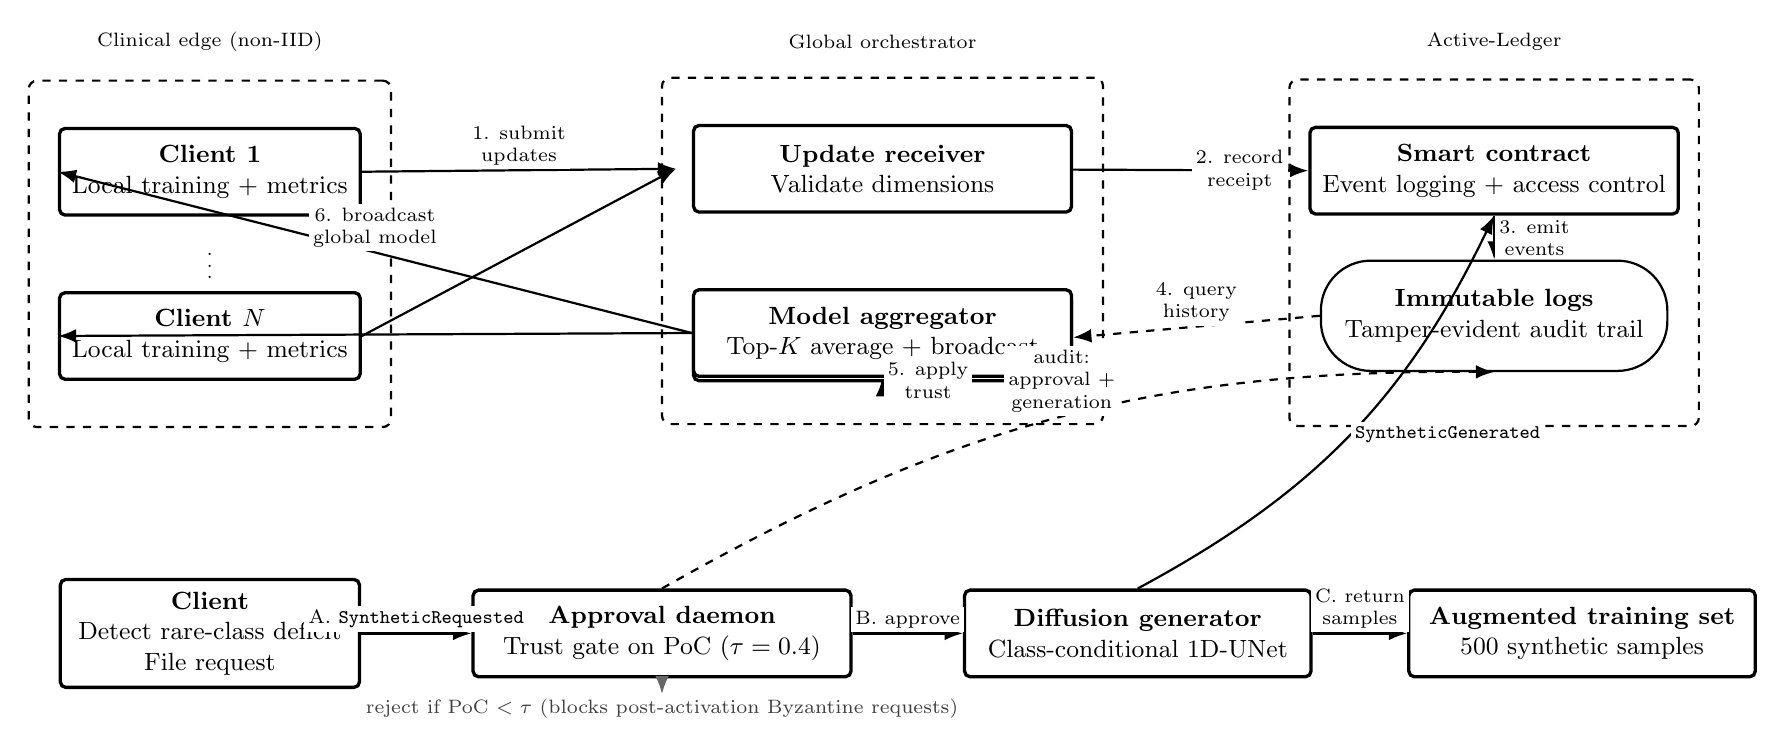
\begin{tikzpicture}[
  font=\small,
  node distance=7mm and 10mm,
  >=Latex,
  box/.style={draw, rounded corners=2pt, very thick, inner sep=4.5pt, align=center, fill=white},
  pill/.style={draw, rounded corners=18pt, thick, inner sep=4pt, align=center, fill=white},
  group/.style={draw, rounded corners=3pt, dashed, thick, inner sep=6pt, fill=white},
  arrow/.style={-Latex, thick},
  garrow/.style={-Latex, thick, dashed},
  lab/.style={font=\scriptsize, align=center, fill=white, inner sep=1.5pt}
]

% --- Column headings (three groups) -----------------------------------------
\node[lab, text=black] (h1) {Clinical edge (non-IID)};
\node[lab, text=black, right=58mm of h1] (h2) {Global orchestrator};
\node[lab, text=black, right=56mm of h2] (h3) {Active-Ledger};

% --- Groups (dashed containers) ---------------------------------------------
\node[group, below=3mm of h1, minimum width=46mm, minimum height=44mm] (gEdge) {};
\node[group, below=3mm of h2, minimum width=56mm, minimum height=44mm] (gOrch) {};
\node[group, below=3mm of h3, minimum width=52mm, minimum height=44mm] (gLedg) {};

% --- Edge nodes --------------------------------------------------------------
\node[box, anchor=north, minimum width=38mm, minimum height=11mm] (c1) at ([yshift=-6mm]gEdge.north) {\textbf{Client 1}\\Local training + metrics};
\node[lab, anchor=north] (dots) at ([yshift=-2mm]c1.south) {$\vdots$};
\node[box, anchor=south, minimum width=38mm, minimum height=11mm] (cN) at ([yshift=6mm]gEdge.south) {\textbf{Client $N$}\\Local training + metrics};

% --- Orchestrator nodes ------------------------------------------------------
\node[box, anchor=north, minimum width=48mm, minimum height=11mm] (recv) at ([yshift=-6mm]gOrch.north) {\textbf{Update receiver}\\Validate dimensions};
\node[box, below=10mm of recv, minimum width=48mm, minimum height=11mm] (poc) {\textbf{PoC engine}\\Compute trust scores};
\node[box, anchor=south, minimum width=48mm, minimum height=11mm] (agg) at ([yshift=6mm]gOrch.south) {\textbf{Model aggregator}\\Top-$K$ average + broadcast};

% --- Ledger nodes ------------------------------------------------------------
\node[box, anchor=north, minimum width=44mm, minimum height=11mm] (sc) at ([yshift=-6mm]gLedg.north) {\textbf{Smart contract}\\Event logging + access control};
\node[pill, anchor=south, minimum width=44mm, minimum height=14mm] (log) at ([yshift=7mm]gLedg.south) {\textbf{Immutable logs}\\Tamper-evident audit trail};

% --- Top flow: aggregation ---------------------------------------------------
\draw[arrow] (c1.east) -- node[lab, above] {1. submit\\updates} ([xshift=-2mm]recv.west);
\draw[arrow] (cN.east) -- ([xshift=-2mm]recv.west);

\draw[arrow] (recv) -- node[lab, right] {2. record\\receipt} (sc.west);
\draw[arrow] (sc) -- node[lab, right] {3. emit\\events} (log.north);

\draw[garrow] (log.west) -- node[lab, above] {4. query\\history} (poc.east);
\draw[arrow] (poc) -- node[lab, right] {5. apply\\trust} (agg);

\draw[arrow] (agg.west) -- node[lab, above] {6. broadcast\\global model} (c1.west);
\draw[arrow] (agg.west) -- (cN.west);

% --- Bottom flow: trust-gated augmentation (separate row) --------------------
\node[box, below=19mm of gEdge.south, minimum width=38mm, minimum height=11mm] (req) {\textbf{Client}\\Detect rare-class deficit\\File request};
\node[box, right=14mm of req, minimum width=48mm, minimum height=11mm] (gate) {\textbf{Approval daemon}\\Trust gate on PoC ($\tau=0.4$)};
\node[box, right=14mm of gate, minimum width=44mm, minimum height=11mm] (gen) {\textbf{Diffusion generator}\\Class-conditional 1D-UNet};
\node[box, right=12mm of gen, minimum width=44mm, minimum height=11mm] (aug) {\textbf{Augmented training set}\\$500$ synthetic samples};

\draw[arrow] (req) -- node[lab, above] {A. \texttt{SyntheticRequested}} (gate);
\draw[garrow] (gate.north) to[bend left=15] node[lab, above] {audit:\\approval +\\generation} (log.south);
\draw[arrow] (gate) -- node[lab, above] {B. approve} (gen);
\draw[arrow] (gen) -- node[lab, above] {C. return\\samples} (aug);
\draw[arrow] (gen.north) to[bend right=18] node[lab, right] {\texttt{SyntheticGenerated}} (sc.south);

% --- Explicit reject path (kept minimal, no clutter) -------------------------
\node[lab, text=black!75, below=2mm of gate.south] (rej) {reject if PoC $<\tau$ (blocks post-activation Byzantine requests)};
\draw[-Latex, thick, black!60] ([yshift=-1mm]gate.south) -- (rej.north);

\end{tikzpicture}


%
% Design goals:
% - LNCS margin-safe (wrapped in \resizebox{...}{!}{...} by the caller)
% - Uncluttered: two horizontal flows (aggregation on top, augmentation below)
% - Close in structure to the provided reference diagram, but with clearer spacing
%
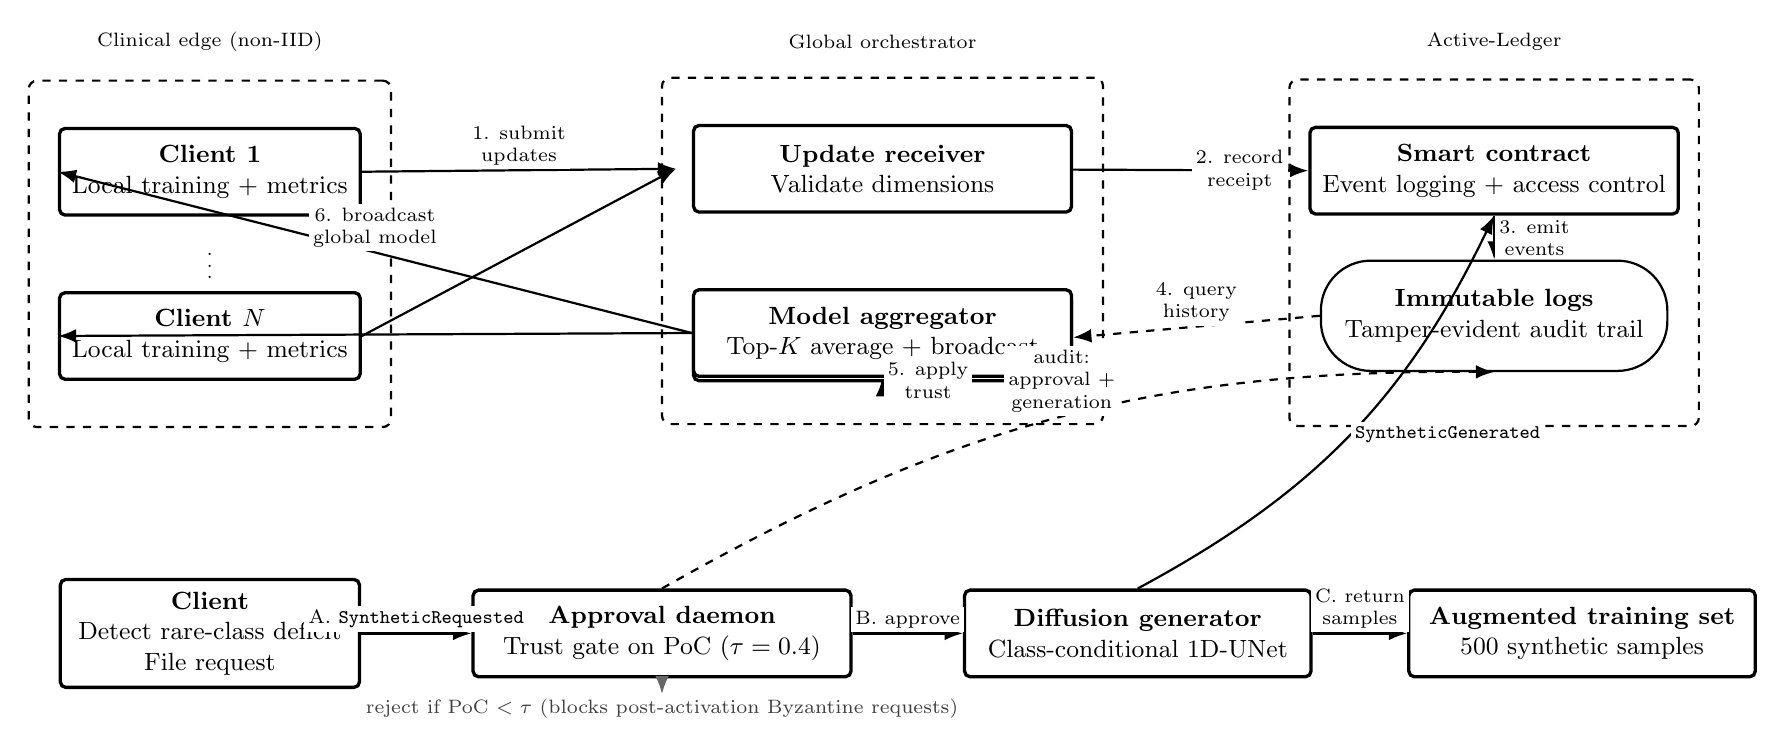
\begin{tikzpicture}[
  font=\small,
  node distance=7mm and 10mm,
  >=Latex,
  box/.style={draw, rounded corners=2pt, very thick, inner sep=4.5pt, align=center, fill=white},
  pill/.style={draw, rounded corners=18pt, thick, inner sep=4pt, align=center, fill=white},
  group/.style={draw, rounded corners=3pt, dashed, thick, inner sep=6pt, fill=white},
  arrow/.style={-Latex, thick},
  garrow/.style={-Latex, thick, dashed},
  lab/.style={font=\scriptsize, align=center, fill=white, inner sep=1.5pt}
]

% --- Column headings (three groups) -----------------------------------------
\node[lab, text=black] (h1) {Clinical edge (non-IID)};
\node[lab, text=black, right=58mm of h1] (h2) {Global orchestrator};
\node[lab, text=black, right=56mm of h2] (h3) {Active-Ledger};

% --- Groups (dashed containers) ---------------------------------------------
\node[group, below=3mm of h1, minimum width=46mm, minimum height=44mm] (gEdge) {};
\node[group, below=3mm of h2, minimum width=56mm, minimum height=44mm] (gOrch) {};
\node[group, below=3mm of h3, minimum width=52mm, minimum height=44mm] (gLedg) {};

% --- Edge nodes --------------------------------------------------------------
\node[box, anchor=north, minimum width=38mm, minimum height=11mm] (c1) at ([yshift=-6mm]gEdge.north) {\textbf{Client 1}\\Local training + metrics};
\node[lab, anchor=north] (dots) at ([yshift=-2mm]c1.south) {$\vdots$};
\node[box, anchor=south, minimum width=38mm, minimum height=11mm] (cN) at ([yshift=6mm]gEdge.south) {\textbf{Client $N$}\\Local training + metrics};

% --- Orchestrator nodes ------------------------------------------------------
\node[box, anchor=north, minimum width=48mm, minimum height=11mm] (recv) at ([yshift=-6mm]gOrch.north) {\textbf{Update receiver}\\Validate dimensions};
\node[box, below=10mm of recv, minimum width=48mm, minimum height=11mm] (poc) {\textbf{PoC engine}\\Compute trust scores};
\node[box, anchor=south, minimum width=48mm, minimum height=11mm] (agg) at ([yshift=6mm]gOrch.south) {\textbf{Model aggregator}\\Top-$K$ average + broadcast};

% --- Ledger nodes ------------------------------------------------------------
\node[box, anchor=north, minimum width=44mm, minimum height=11mm] (sc) at ([yshift=-6mm]gLedg.north) {\textbf{Smart contract}\\Event logging + access control};
\node[pill, anchor=south, minimum width=44mm, minimum height=14mm] (log) at ([yshift=7mm]gLedg.south) {\textbf{Immutable logs}\\Tamper-evident audit trail};

% --- Top flow: aggregation ---------------------------------------------------
\draw[arrow] (c1.east) -- node[lab, above] {1. submit\\updates} ([xshift=-2mm]recv.west);
\draw[arrow] (cN.east) -- ([xshift=-2mm]recv.west);

\draw[arrow] (recv) -- node[lab, right] {2. record\\receipt} (sc.west);
\draw[arrow] (sc) -- node[lab, right] {3. emit\\events} (log.north);

\draw[garrow] (log.west) -- node[lab, above] {4. query\\history} (poc.east);
\draw[arrow] (poc) -- node[lab, right] {5. apply\\trust} (agg);

\draw[arrow] (agg.west) -- node[lab, above] {6. broadcast\\global model} (c1.west);
\draw[arrow] (agg.west) -- (cN.west);

% --- Bottom flow: trust-gated augmentation (separate row) --------------------
\node[box, below=19mm of gEdge.south, minimum width=38mm, minimum height=11mm] (req) {\textbf{Client}\\Detect rare-class deficit\\File request};
\node[box, right=14mm of req, minimum width=48mm, minimum height=11mm] (gate) {\textbf{Approval daemon}\\Trust gate on PoC ($\tau=0.4$)};
\node[box, right=14mm of gate, minimum width=44mm, minimum height=11mm] (gen) {\textbf{Diffusion generator}\\Class-conditional 1D-UNet};
\node[box, right=12mm of gen, minimum width=44mm, minimum height=11mm] (aug) {\textbf{Augmented training set}\\$500$ synthetic samples};

\draw[arrow] (req) -- node[lab, above] {A. \texttt{SyntheticRequested}} (gate);
\draw[garrow] (gate.north) to[bend left=15] node[lab, above] {audit:\\approval +\\generation} (log.south);
\draw[arrow] (gate) -- node[lab, above] {B. approve} (gen);
\draw[arrow] (gen) -- node[lab, above] {C. return\\samples} (aug);
\draw[arrow] (gen.north) to[bend right=18] node[lab, right] {\texttt{SyntheticGenerated}} (sc.south);

% --- Explicit reject path (kept minimal, no clutter) -------------------------
\node[lab, text=black!75, below=2mm of gate.south] (rej) {reject if PoC $<\tau$ (blocks post-activation Byzantine requests)};
\draw[-Latex, thick, black!60] ([yshift=-1mm]gate.south) -- (rej.north);

\end{tikzpicture}

%
}
\caption{The two flows of \actledger. The top half is the
aggregation pipeline: clients train locally and upload updates, the
server ranks them by their PoC score and averages the top seven, and
every step leaves a receipt on the ledger. The bottom half is the
trust-gated augmentation pipeline: a client that detects rare-class
deficit files an on-chain request, the approval daemon either
approves or rejects based on PoC, and only approved requests reach
the diffusion generator.}
\label{fig:architecture}
\end{figure}

% ============================================================================
\section{Threat Model}
\label{sec:threat}

Two of the ten clients are Byzantine in every experiment; the other
eight are identical across all runs, so that any performance
difference is due to the defence and the attack, not the honest
silos. Three attack strategies on aggregation and one on augmentation
are considered.

\paragraph{Gaussian weight poisoning.}
In the simplest attack, a Byzantine client replaces its uploaded
weight tensor with pure uniform noise at every round. This is the
canonical sanity-check attack used in the original Byzantine-FL
papers~\cite{blanchard2017krum,elmhamdi2018bulyan}. It is not
stealthy and any serious robust aggregator should reject it; its
role in the experimental grid is to establish a lower bound on how
\fedavg behaves when no defence is present.

\paragraph{Static semantic label-flip.}
In a stealthier attack, the Byzantine client trains honestly on
corrupted labels. Before each local batch it applies a targeted
pairwise flip between Normal (Class 0) and LBBB (Class 1) -- every
Normal sample is relabelled LBBB and every LBBB sample is relabelled
Normal -- while the other three classes are left untouched. The two
Byzantine clients truncate their poisoned batches to the same length
so their flipped-label gradients cluster tightly together (colluding
rather than drifting apart). The attacker then runs ordinary local
training on these wrong labels and uploads the resulting weights.
The uploaded gradients have perfectly normal magnitudes and
directions -- they are a valid training step on some data -- so only
the target semantics are poisoned, and distance-based aggregators
cannot easily distinguish them from honest non-IID updates.

\paragraph{Sleeper backdoor-critical-layer flip.}
The most interesting attack is the sleeper, motivated by Zhuang et
al.~\cite{zhuang2024bclayers} and Foroughi et
al.~\cite{foroughi2026lsa}. Each Byzantine client behaves honestly
for the first fifteen rounds and then activates a targeted backdoor
that relabels APB (Class 3) as LBBB (Class 1). Rather than retrain
the whole model on these poisoned samples, the attacker freezes all
weights except a small set of backdoor-critical layers at the tail of
the classifier, fine-tunes only those layers on the relabelled APB
data, and uploads a crafted update in which the non-critical layers
are left identical to the current global model. Unlike data-poisoning
backdoors that inject a physical waveform trigger into the ECG
itself, this is purely a semantic backdoor: the raw waveforms remain
morphologically pristine and only the learned mapping from the APB
manifold to the APB label is corrupted, which is why distance-based
aggregators that look only at weight-vector geometry cannot separate
it from the drift of an honest non-IID update. Round fifteen is
chosen empirically as the point at which vanilla \fedavg on the
substrate used here has already reached a healthy global model (macro-F1
around $0.90$, APB-F1 around $0.75$), so the attackers have
accumulated a good-citizen history and no per-round rule has any
signal to latch onto in the early rounds.

\paragraph{Augmentation stealth bypass.}
In the diffusion-augmented setting, the sleeper attacker
additionally participates in the synthetic-data pipeline. A
malicious request looks like a valid rare-class request on-chain,
but the class label inside the request has been flipped. If the
generator is not gated, this causes the UNet to denoise into the
LBBB manifold while the request is stamped as APB, so the
attacker-chosen label is injected into the local training set
together with synthetic samples from the wrong class. The PoC gate
is designed to block this channel: once the EMA picks up the
post-activation accuracy drop, the attacker's PoC falls below the
trust threshold and its requests stop being approved.

% ============================================================================
\section{Defences and Methods}
\label{sec:methods}

\subsection{Aggregation rules under comparison}
\label{subsec:defences}
The experiments use ten clients with two assumed Byzantines
throughout. The seven defences under comparison differ only in how
they aggregate the uploaded updates.
\begin{description}
\item[\fedavg~\cite{mcmahan2017fedavg}.] The new global model is the
sample-size-weighted mean of all uploaded updates, with no attack
filtering.
\item[\krum~\cite{blanchard2017krum}.] The server picks the single
client whose squared distance to its closest neighbours is minimal,
and uses that client's update as the new global model.
\item[\mkrum.] Same scoring as \krum, but the server averages
several lowest-scored clients rather than picking one.
\item[\median~\cite{yin2018byzantine}.] The new global model is the
coordinate-wise median of all uploaded updates.
\item[\tmean~\cite{yin2018byzantine}.] For each coordinate, the top
and bottom twenty percent of the uploaded values are dropped and the
rest averaged.
\item[\bulyan~\cite{elmhamdi2018bulyan}.] A \mkrum pre-filter is
applied first, and the survivors are aggregated coordinate-wise by
\tmean.
\item[\poc (this work).] Clients are ranked by the PoC score of
Eq.~\eqref{eq:poc} and the top seven are averaged weighted by their
local sample sizes.
\end{description}
The first six rules are per-round geometric filters; \poc is the only
behavioural rule in the set.

\subsection{Trust-gated diffusion}
The augmentation comparison uses a class-conditional 1D-UNet latent
diffusion generator~\cite{ho2020ddpm,rombach2022ldm}. The
model is pre-trained once, before FL begins, on pooled honest-client
ECG windows (no test-set windows are ever shown to the generator),
and its weights are frozen during the federated schedule -- only
inference runs during training. Conditioning is by channel
concatenation: the integer class label is normalised to the unit
interval, broadcast along the time axis, and concatenated to the
noisy ECG window as a second input channel. Inference uses thirty
DDPM steps, which is the smallest number at which clinically
plausible QRS morphology is still observed. Two policies are
compared.
\begin{description}
\item[\tgldm (this work).] A synthetic-data request is approved
only when the requester's PoC score is at least the trust threshold
of $0.4$ from Section~\ref{subsec:poc}.
\item[\bldm.] A synthetic-data request is granted unconditionally.
This policy is paired with \mkrum on the aggregation side so that
the comparison is a fair test of what the ledger adds once a robust
aggregator is already in place.
\end{description}

\subsection{Metrics}
\label{subsec:metrics}
MIT-BIH is heavily imbalanced, so the per-class F1 on APB
(Class 3) is adopted as the primary clinical metric and denoted
APB-F1; macro-F1 is reported as a secondary consistency metric. The
diffusion experiments additionally report the backdoor success rate
(BSR), defined as the fraction of APB-targeted trigger samples that
the global classifier assigns to the attacker-chosen non-APB label;
lower BSR is better. Per-round training latencies fall in the twenty
to twenty-seven second range for the non-diffusion methods, with
\poc adding a single-digit percent overhead over \mkrum due to
on-chain logging. Latency is not a contribution of this paper; it is
mentioned only to show that the ledger is not a wall-clock drag.

% ============================================================================
\section{Experimental Setup}
\label{sec:setup}

All experiments use the MIT-BIH Arrhythmia Database~%
\cite{moody2001mitbih} preprocessed under the AAMI EC57
protocol~\cite{aami1998ec57}. Each heartbeat is segmented into a
360-sample window at 360\,Hz and normalised to zero mean and unit
variance. Every client splits its local data into train (70\%),
validation (15\%) and test (15\%); the held-out 15\% is used only
for the final per-class classification report. All runs execute on
a single T4 GPU with a Ganache v7 in-process Ethereum chain. The
shared hyper-parameters are ten clients (two Byzantine), forty
global rounds, three local epochs per round, batch size 128, Adam
with learning rate $10^{-3}$, and Dirichlet concentration $0.5$.
Every cell of the grid serialises the per-round macro-F1, per-class
F1, final classification report and per-round latency, and the
diffusion cells additionally serialise per-round APB-F1 and per-round
BSR; the numbers quoted throughout the paper are extracted
programmatically from these artefacts so that figures, tables and
prose remain internally consistent.

% ============================================================================
\section{Results}
\label{sec:results}

The rare-class metric across all three aggregation attacks is
examined first; that already decides the primary claim. Macro-F1 on
the same grid is then inspected to reveal why macro-F1 is the wrong
metric to read alone. The analysis then zooms into the sleeper
attack to see how the defences behave over time, and finally turns
on the diffusion pipeline, compares the trust-gated and blind
policies, and closes with a synthesis figure.

\subsection{Rare-class integrity across attacks}
\label{subsec:apb_heatmap}
Consider the primary metric first. Figure~\ref{fig:apb_heatmap}
reports the final-round APB-F1 for every (defence, attack) cell.
Two failure modes jump out. The first is \fedavg under Gaussian
poisoning: the out-of-distribution uploads dominate the
coordinate-wise mean, the global classifier degenerates into
predicting Normal for every input, and APB-F1 drops to exactly
$0.000$. All four non-Normal per-class F1 scores are zero, and
macro-F1 is flat at $0.1711$ across all forty rounds. The second
failure mode is \krum under the sleeper attack, where APB-F1 ends at
$0.3065$: the post-activation malicious updates look geometrically
normal and \krum has no behavioural signal to tell it that two of
its accepted workers have quietly changed policy.

\begin{figure}[!htbp]
\centering
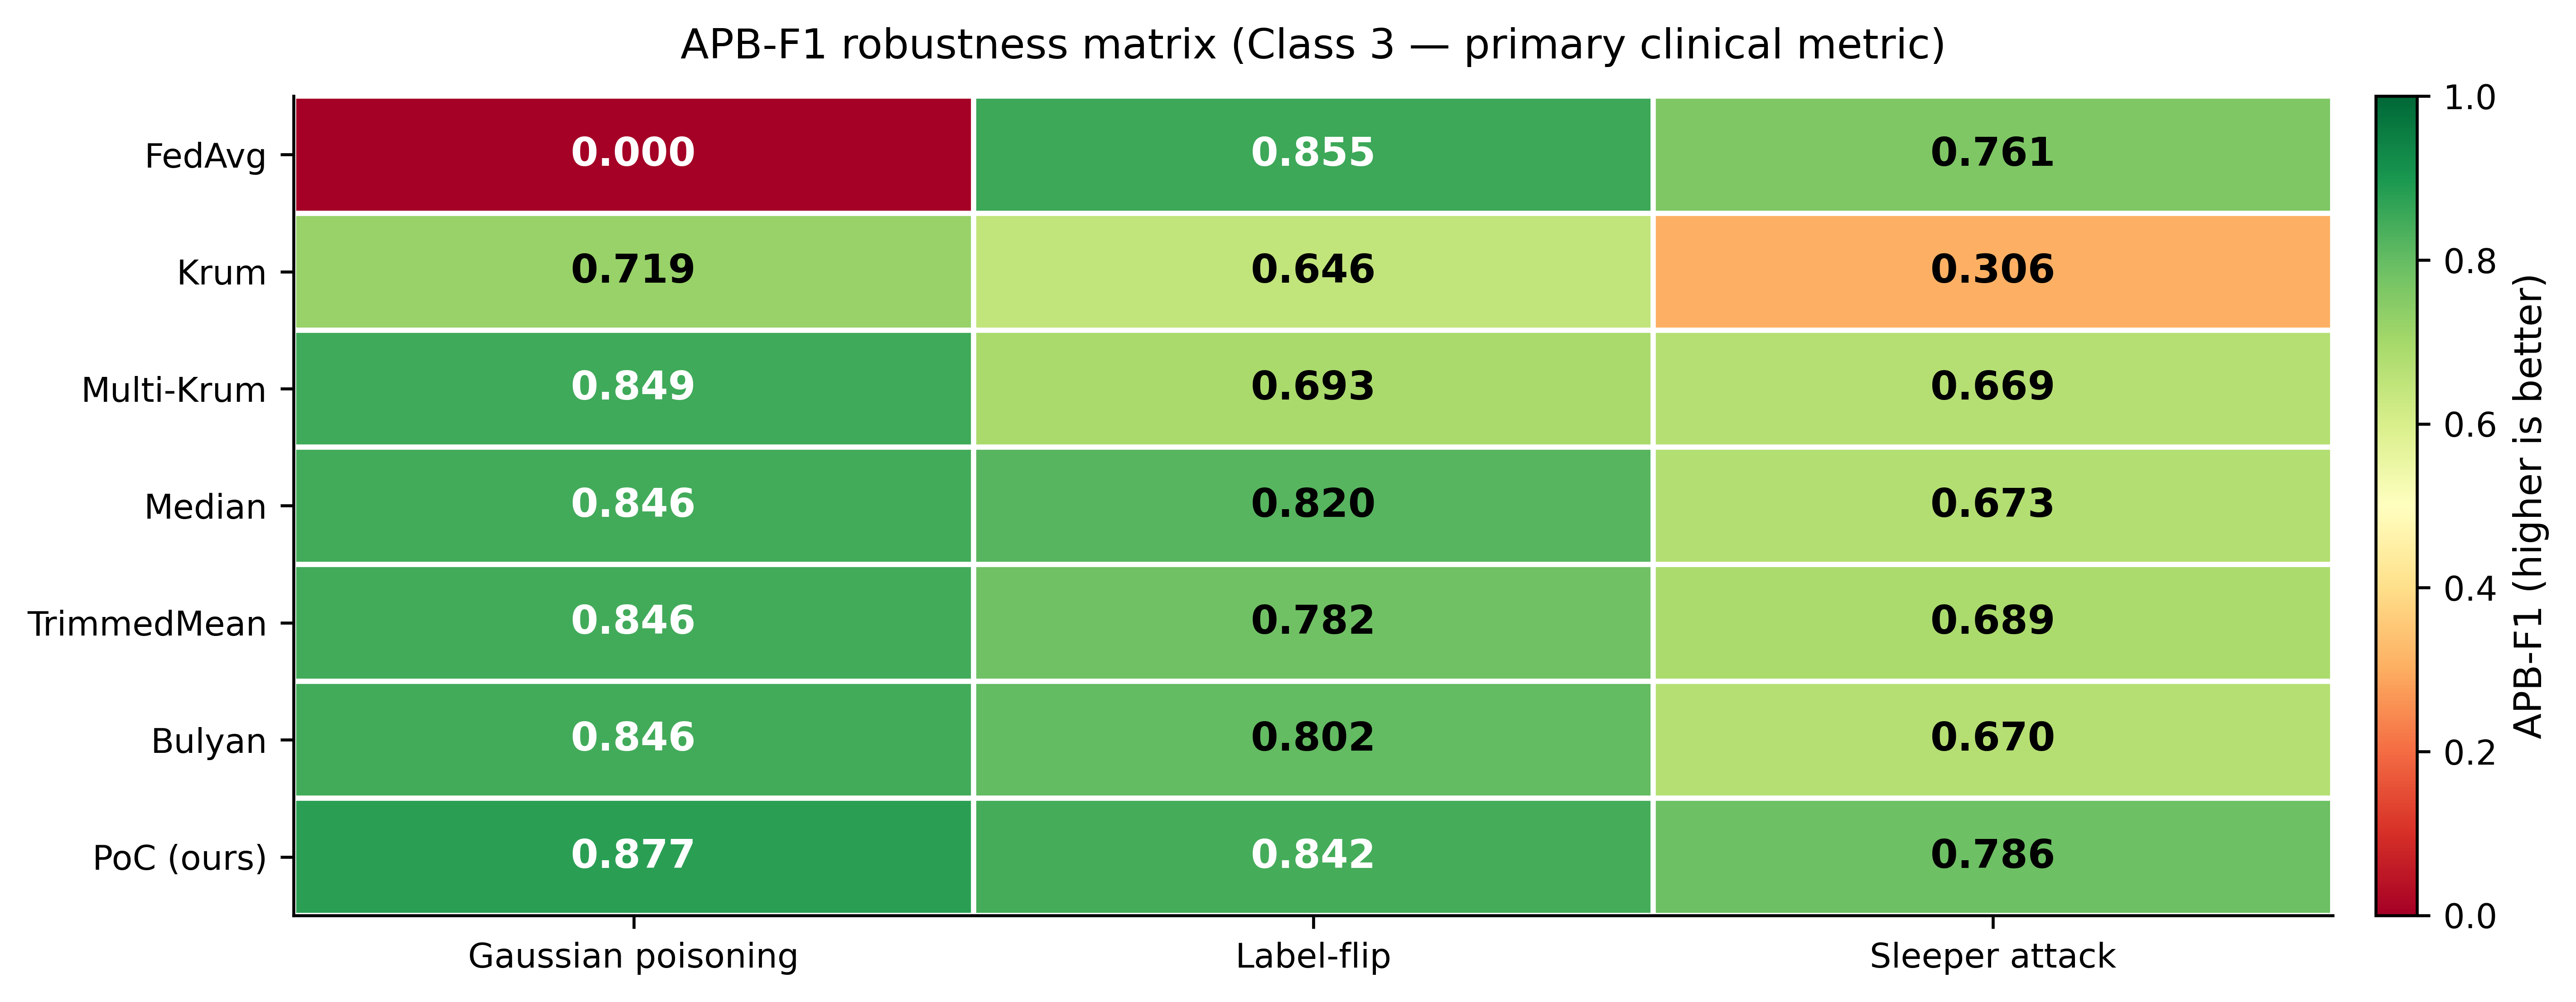
\includegraphics[width=0.94\linewidth]{figures_phase3/fig_apb_heatmap.png}
\caption{APB-F1 on the held-out test set for each of the seven
defences under each of the three attacks. Cells are coloured from
red (low F1) to green (high F1); the $0.75$ line is the clinical
deployability threshold adopted here. \poc is the only defence whose
APB-F1 stays above $0.75$ in every attack: \fedavg collapses under
Gaussian poisoning and \krum collapses under the sleeper attack.}
\label{fig:apb_heatmap}
\end{figure}

The remaining four robust aggregators -- \mkrum, \median, \tmean,
\bulyan -- cluster between APB-F1 around $0.64$ and $0.85$ across
the three attacks. Distance-based filtering clearly helps on the
blatant Gaussian attack, but it gives up ground on the stealthier
semantic and sleeper attacks. As Fig.~\ref{fig:apb_heatmap} shows,
only \poc stays above $0.75$ everywhere, with worst case $0.7858$
(sleeper) and best $0.8773$ (Gaussian). This is the paper's primary
quantitative claim.

\subsection{Why macro-F1 would be misleading here}
\label{subsec:macro_heatmap}
Macro-F1 on the same grid (Fig.~\ref{fig:macro_heatmap}) tells a
different story that is, at face value, misleading: it seems to
suggest that \fedavg is a competitive defence under label-flip
($0.961$) and sleeper ($0.925$). The explanation is a dilution
effect. With a twenty percent attacker ratio and Dirichlet
concentration $0.5$, the honest gradients are themselves diverse,
so the coordinate-wise mean washes the flipped-label signal out on
the four common classes. Distance-based aggregators, in the other
direction, penalise honest non-IID clients whose local distribution
is far from the mean and pay for this on the minority class -- the
one a clinician actually cares about. Macro-F1 is therefore treated
only as a secondary consistency metric, with APB-F1 designated as
the primary metric for the rest of the paper.

\begin{figure}[!htbp]
\centering
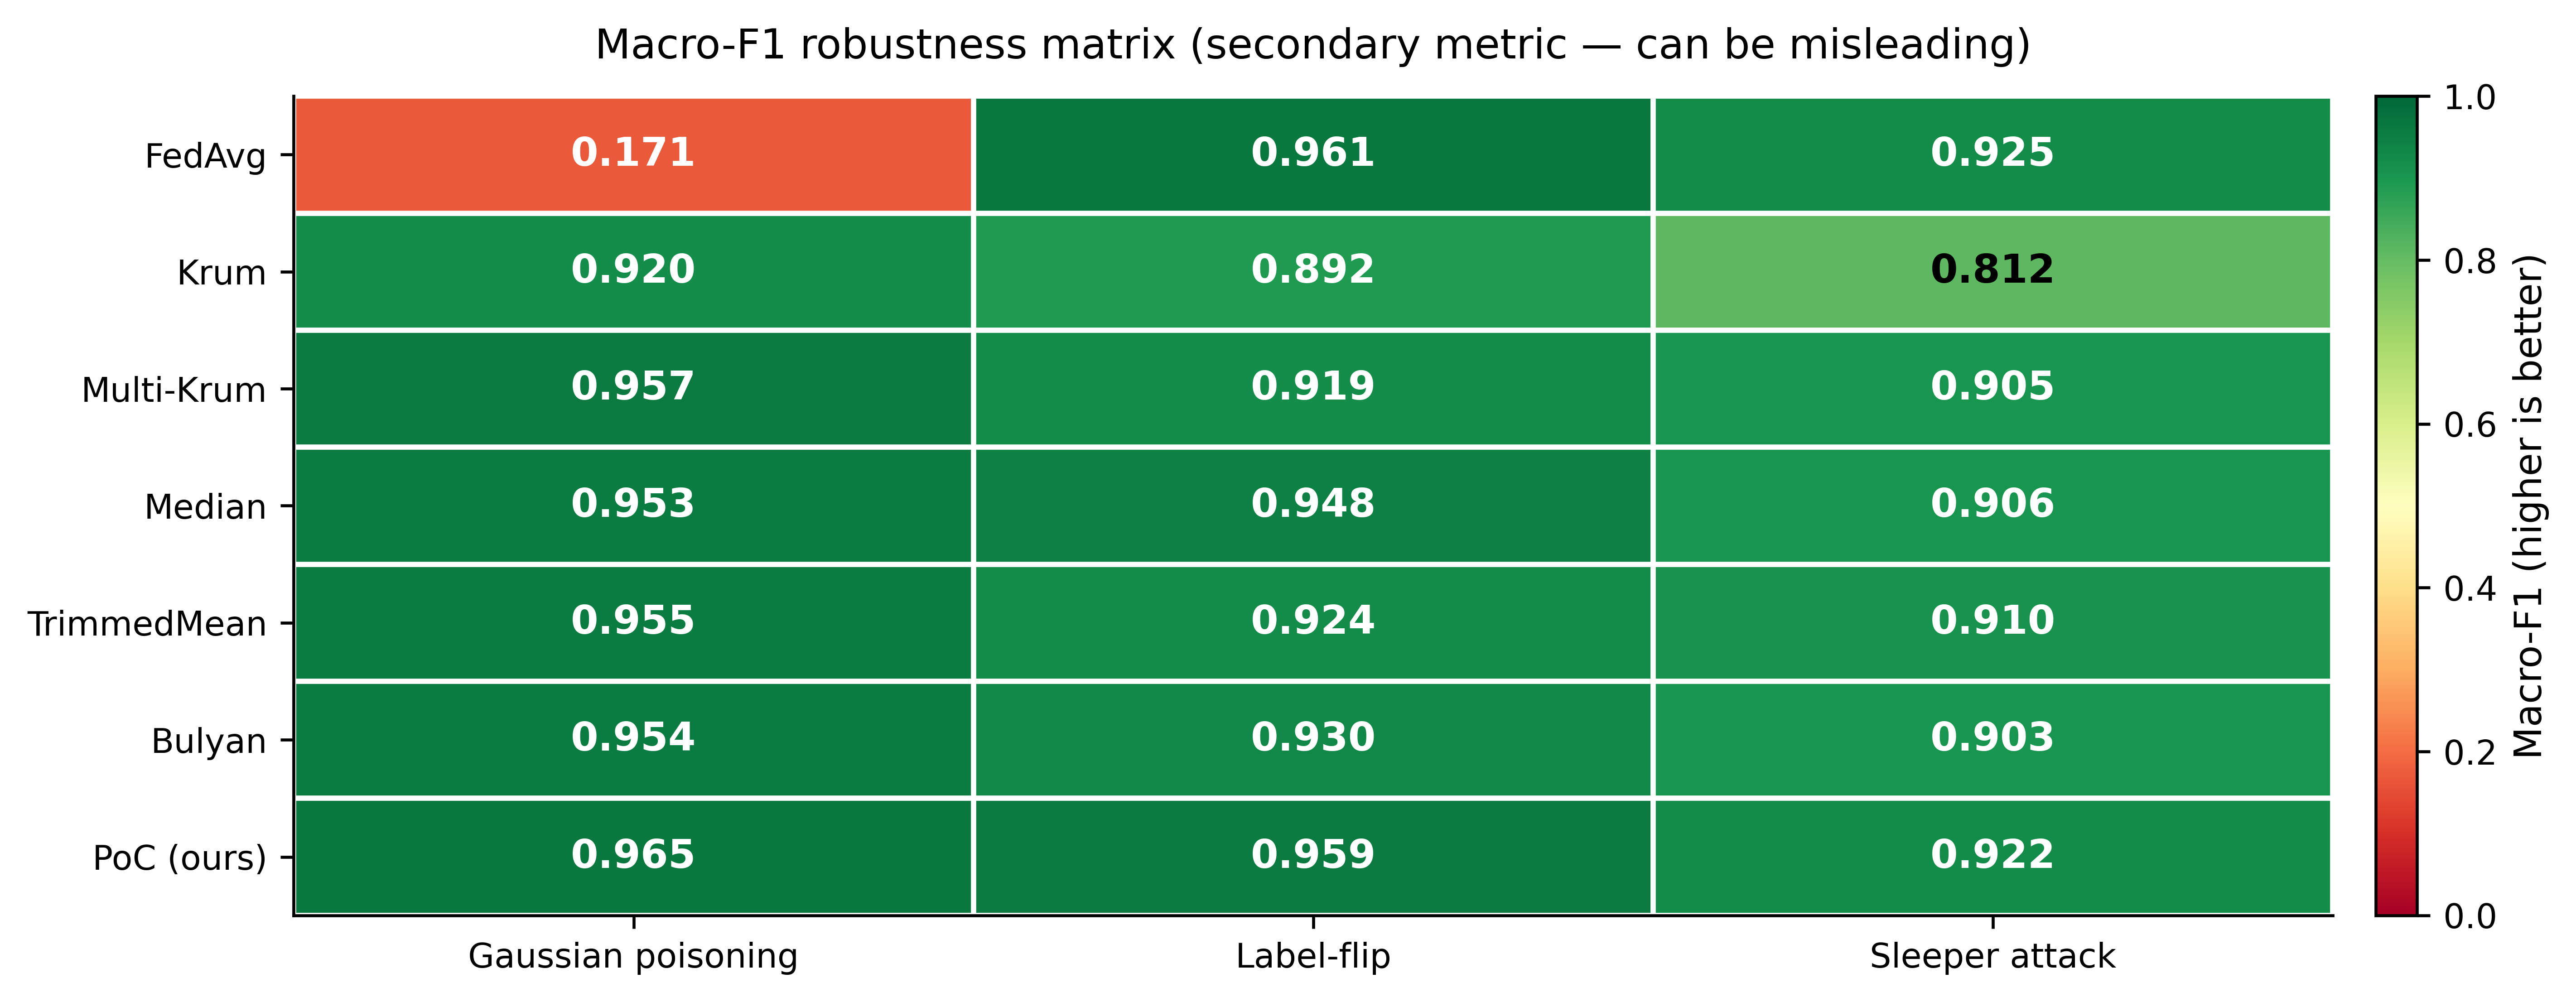
\includegraphics[width=0.94\linewidth]{figures_phase3/fig_macro_heatmap.png}
\caption{Macro-F1 on the same grid as Fig.~\ref{fig:apb_heatmap}.
Taken alone, this matrix would read as if \fedavg is a safe defence
under label-flip and sleeper attacks, which Fig.~\ref{fig:apb_heatmap}
shows is not clinically true.}
\label{fig:macro_heatmap}
\end{figure}

\FloatBarrier

\subsection{Sleeper dynamics: how the attack evolves}
\label{subsec:sleeper}
The final-round numbers do not show how each defence gets there.
Figure~\ref{fig:sleeper} zooms into the sleeper attack and plots, for
four representative defences, macro-F1 over rounds (top panel) and
APB-F1 over rounds (bottom panel). The vertical dotted line marks
the activation round, and the horizontal dashed line on the bottom
panel marks the $0.75$ APB-F1 clinical threshold.

\begin{figure}[!htbp]
\centering
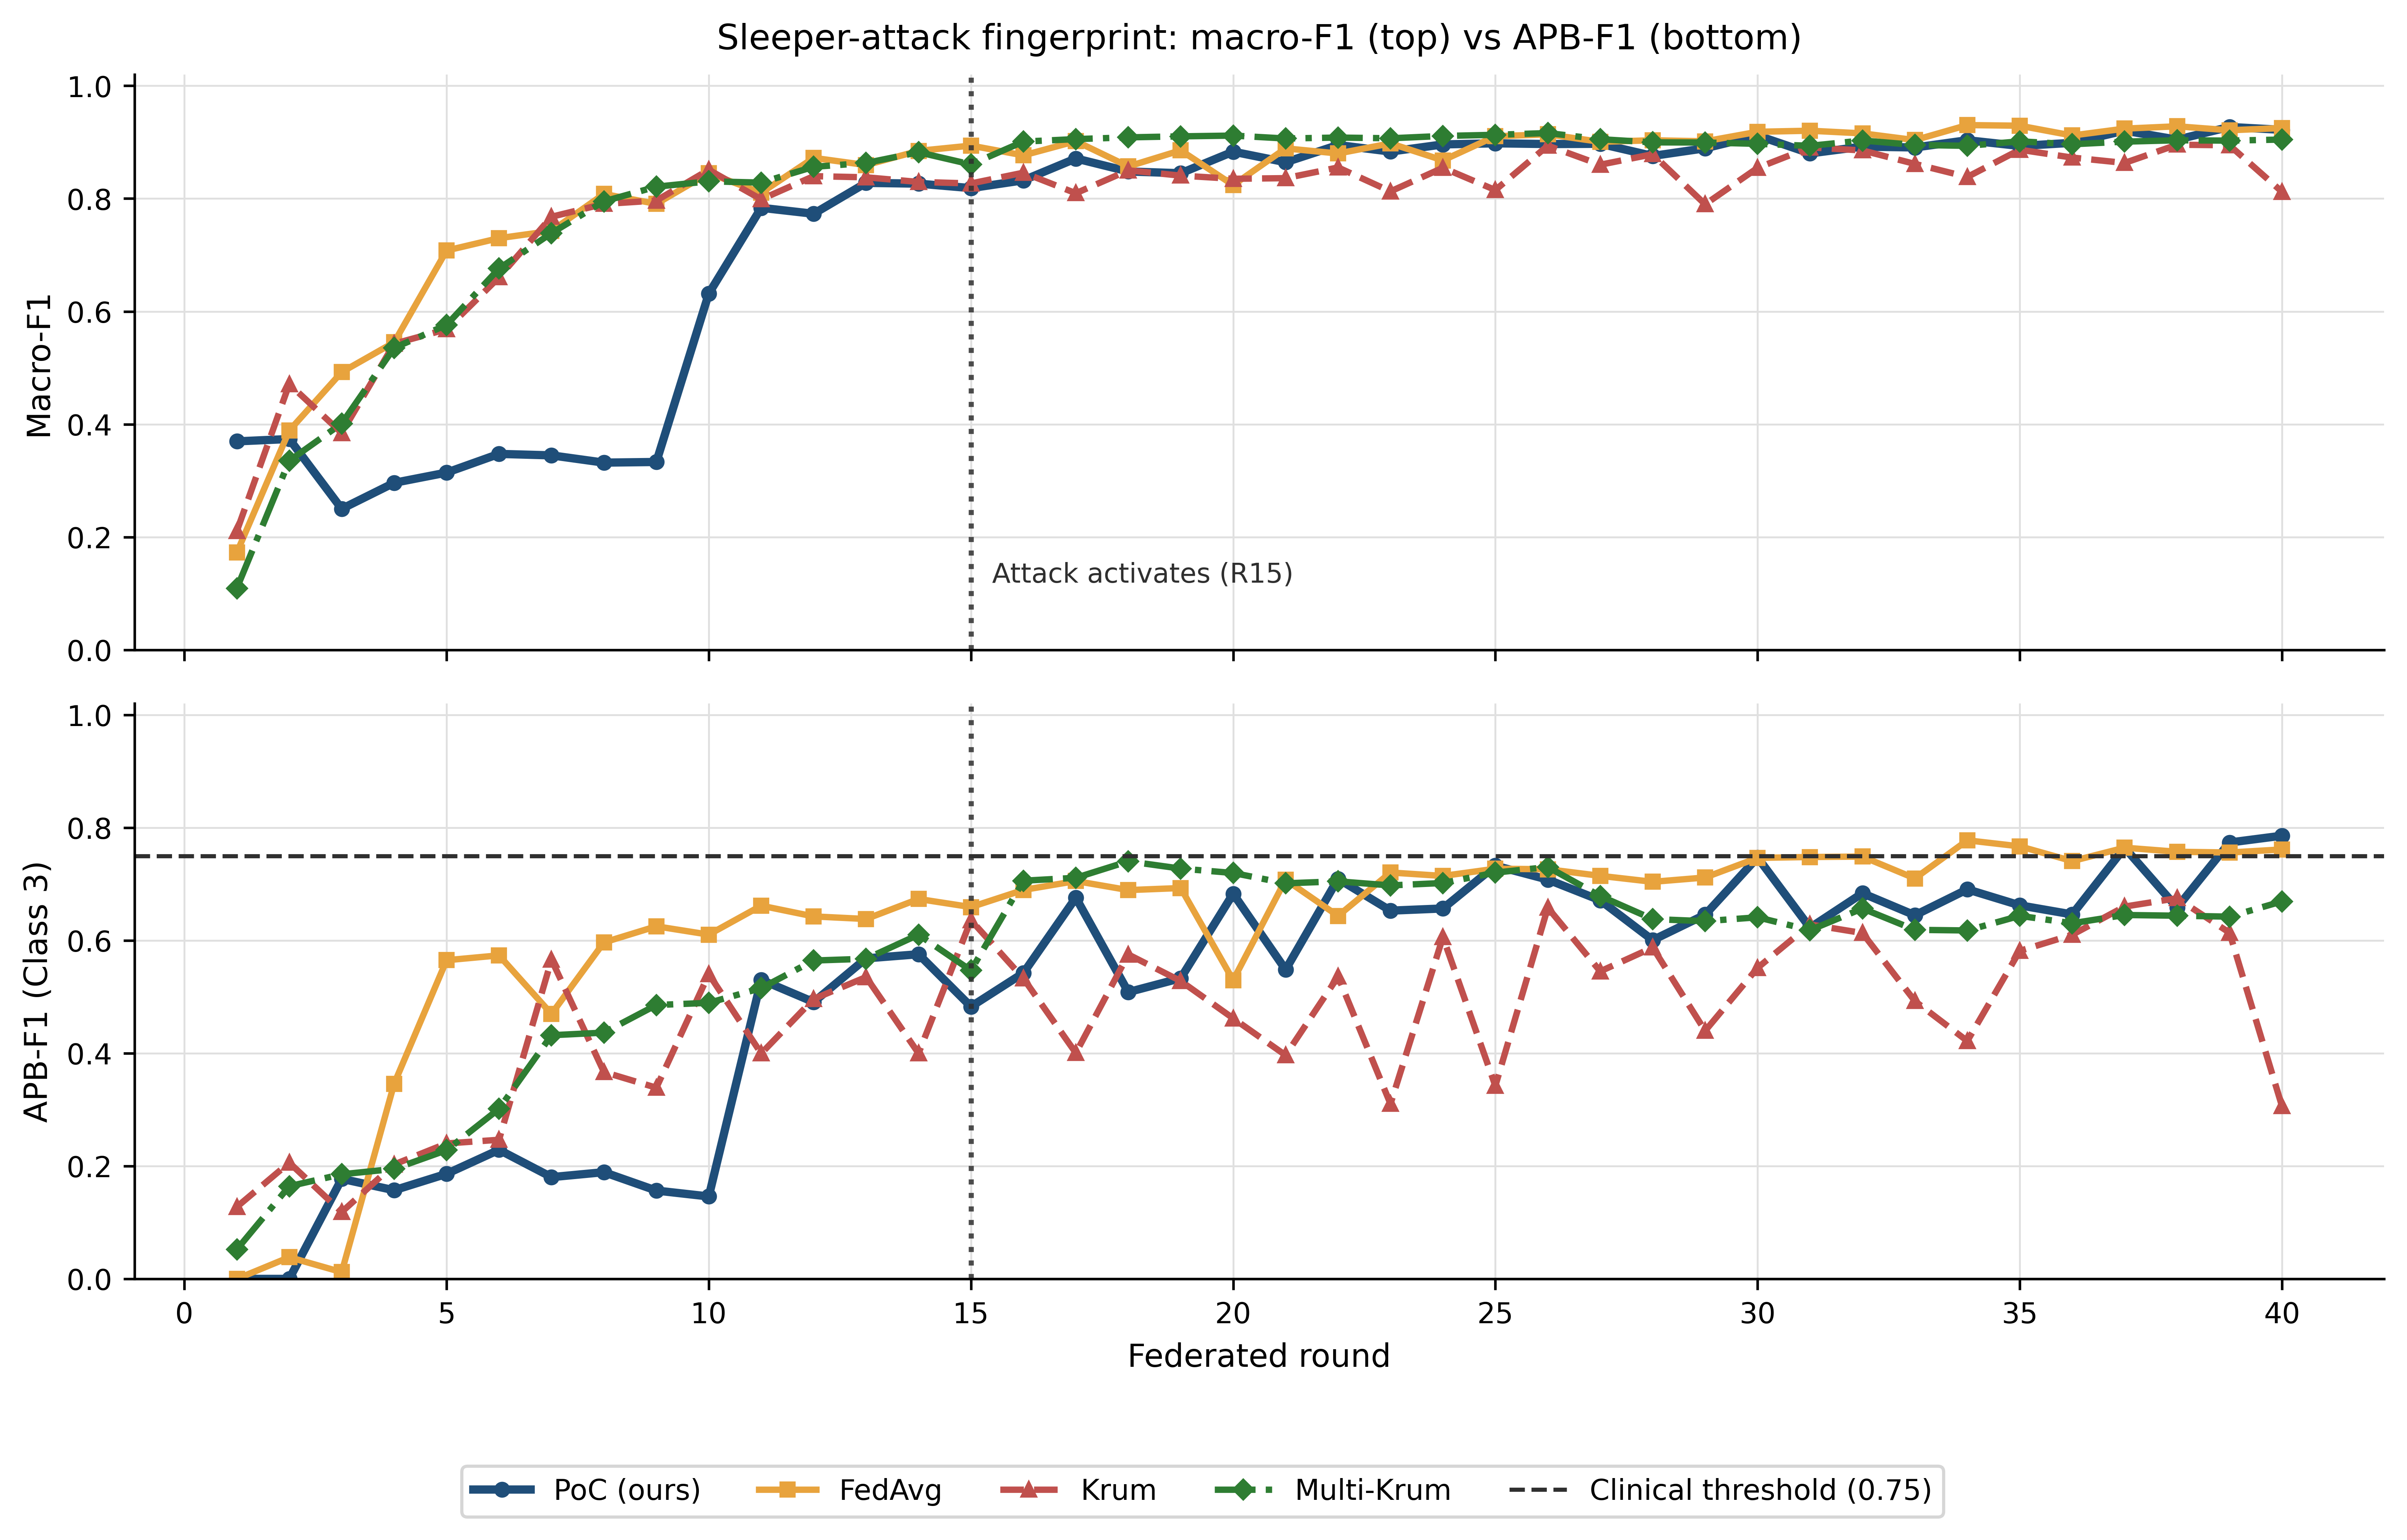
\includegraphics[width=0.94\linewidth]{figures_phase3/fig_sleeper_fingerprint.png}
\caption{Training dynamics of four representative defences under the
sleeper attack. Before activation all four curves are close; after
activation \krum's APB-F1 oscillates and ends near $0.31$, while
\poc stays at or above the $0.75$ threshold by the final rounds.}
\label{fig:sleeper}
\end{figure}

Before activation all four curves are close, which is by design: the
sleeper is engineered to look geometrically normal during the
pre-activation phase. After activation, \krum's APB-F1 begins to
oscillate almost immediately and degrades to $0.3065$ by the final
round, because \krum commits to a single client per round and is
fooled whenever a flipped-label gradient happens to sit close to the
geometric centre on a non-IID batch. \poc recovers within a handful
of rounds as the EMA picks up the attackers' drop in their own
validation accuracy and the attackers fall out of the top seven.
\fedavg and \mkrum end up in between.

\subsection{Trust-gated diffusion under the sleeper}
\label{subsec:ldm_ts}
Turning on the diffusion pipeline changes the picture on both sides.
Figure~\ref{fig:ldm_ts} shows the training dynamics under the
sleeper attack when augmentation is enabled, for two cells: \poc
combined with the trust-gated generator, and \mkrum combined with an
un-gated generator. Both cells rise past the $0.75$ APB-F1 threshold
within a few rounds and both converge above $0.95$ on macro-F1.
Notably, the attack-activation line does not produce a visible
collapse in either curve; the honest diffusion contribution already
stabilises the minority class. But the two cells are not the same:
the trust-gated cell ends with APB-F1 equal to $0.8785$, while the
blind cell ends at $0.8568$, and the gap is consistent from
mid-training onward rather than a single lucky round.

\begin{figure}[!htbp]
\centering
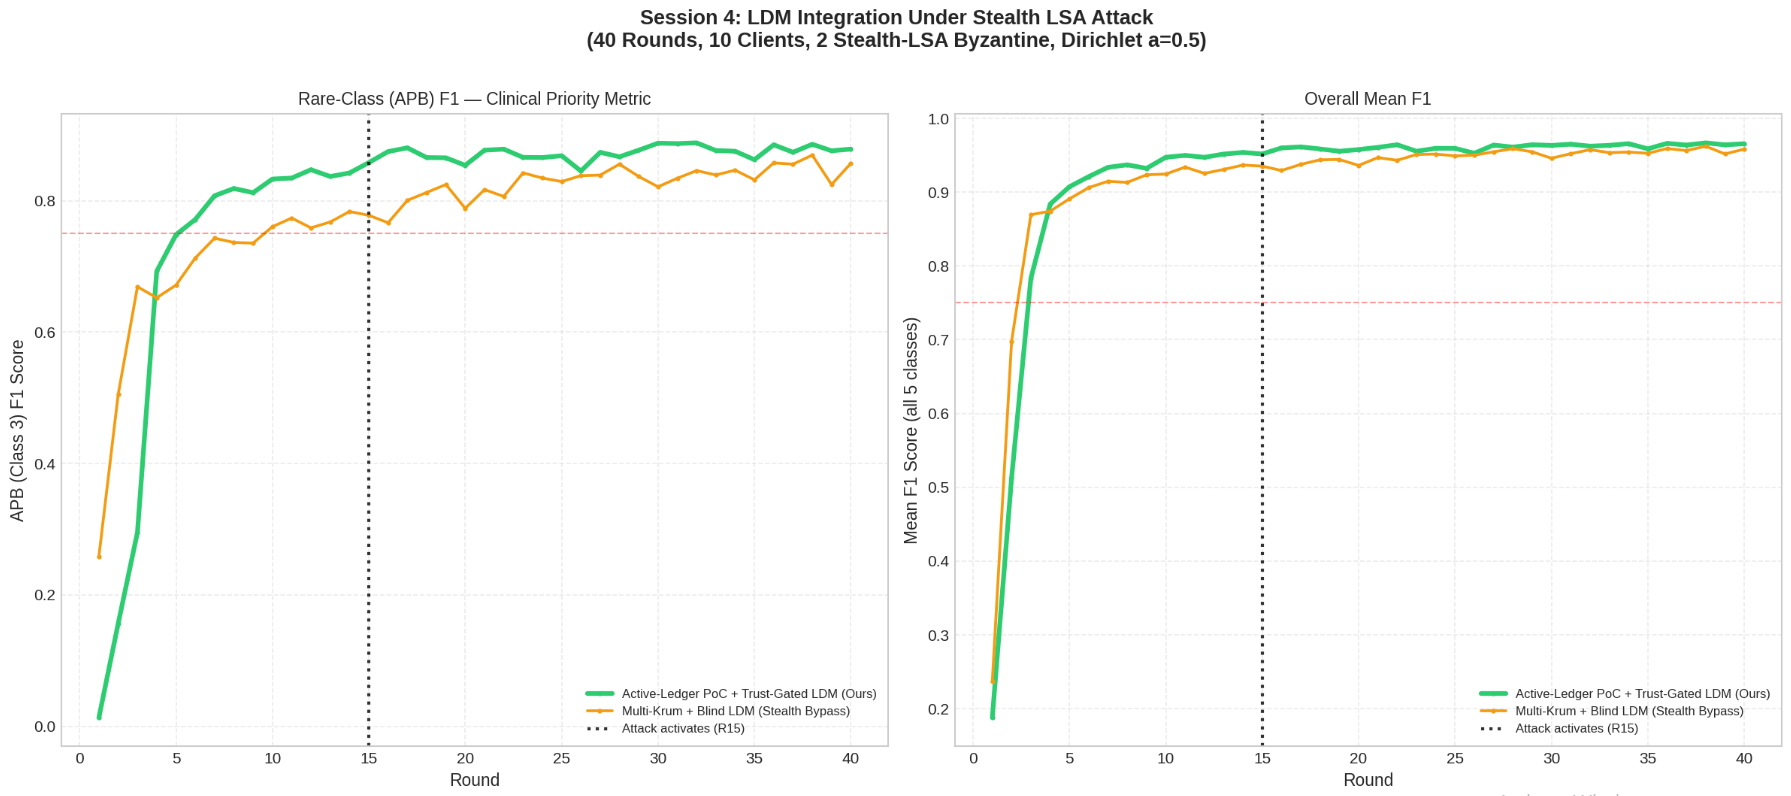
\includegraphics[width=0.94\linewidth]{figures_phase3/image-5.png}
\caption{APB-F1 (left) and macro-F1 (right) over rounds when the
diffusion generator is enabled, under the sleeper attack. The
trust-gated cell (\poc\,+\,\tgldm) is consistently higher than the
blind cell (\mkrum\,+\,\bldm) from mid-training onward.}
\label{fig:ldm_ts}
\end{figure}

\subsection{Backdoor success rate: where the security story hides}
\label{subsec:bsr}
APB-F1 alone does not tell the full story, because a Byzantine
client in the augmented setting can still leak some backdoor
capacity even when APB-F1 looks healthy. The security-relevant
quantity is the backdoor success rate (BSR), plotted in
Fig.~\ref{fig:bsr}. Both cells sit at zero before the attack
activates. After activation both oscillate between roughly $0.05$
and $0.20$ -- the attack is present, and no defence eliminates it
entirely. What differs is the final-round BSR: the blind cell ends
higher than the trust-gated cell. Un-gated diffusion keeps admitting
the attacker's synthetic requests throughout training, while the PoC
gate stops approving them once the behavioural score has caught up
with the attackers' post-activation accuracy drop. The augmentation
receipts on the ledger also make the decision chain inspectable
after the fact: a reviewer can replay exactly which requests were
approved at which PoC score, and by whom.

\begin{figure}[!htbp]
\centering
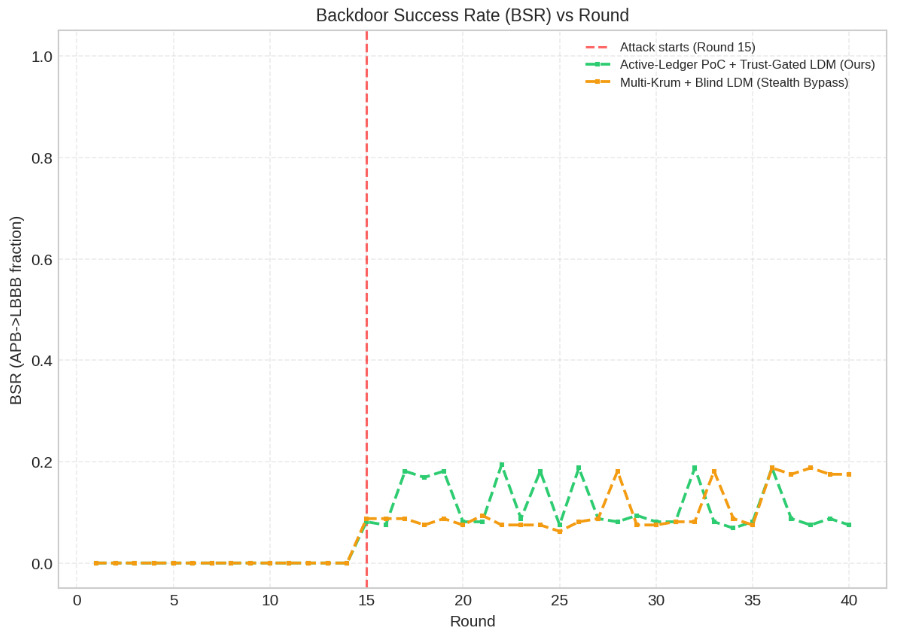
\includegraphics[width=0.78\linewidth]{figures_phase3/image-6.png}
\caption{Backdoor success rate (BSR) per round, under the sleeper
attack. Lower is better. After activation, BSR oscillates in the
$[0.05, 0.20]$ range for both cells, but the blind cell ends at a
higher BSR than the trust-gated cell.}
\label{fig:bsr}
\end{figure}

\subsection{Putting it all together}
\label{subsec:synthesis}
Figure~\ref{fig:synthesis} draws the two halves of the paper into a
single picture. The left block reports, for each defence, its
worst-case APB-F1 across the three attacks -- the number that
matters if a clinical deployment has no control over which attack it
sees. The right block reports the final-round APB-F1 under the two
diffusion-augmented policies.

\begin{figure}[!htbp]
\centering
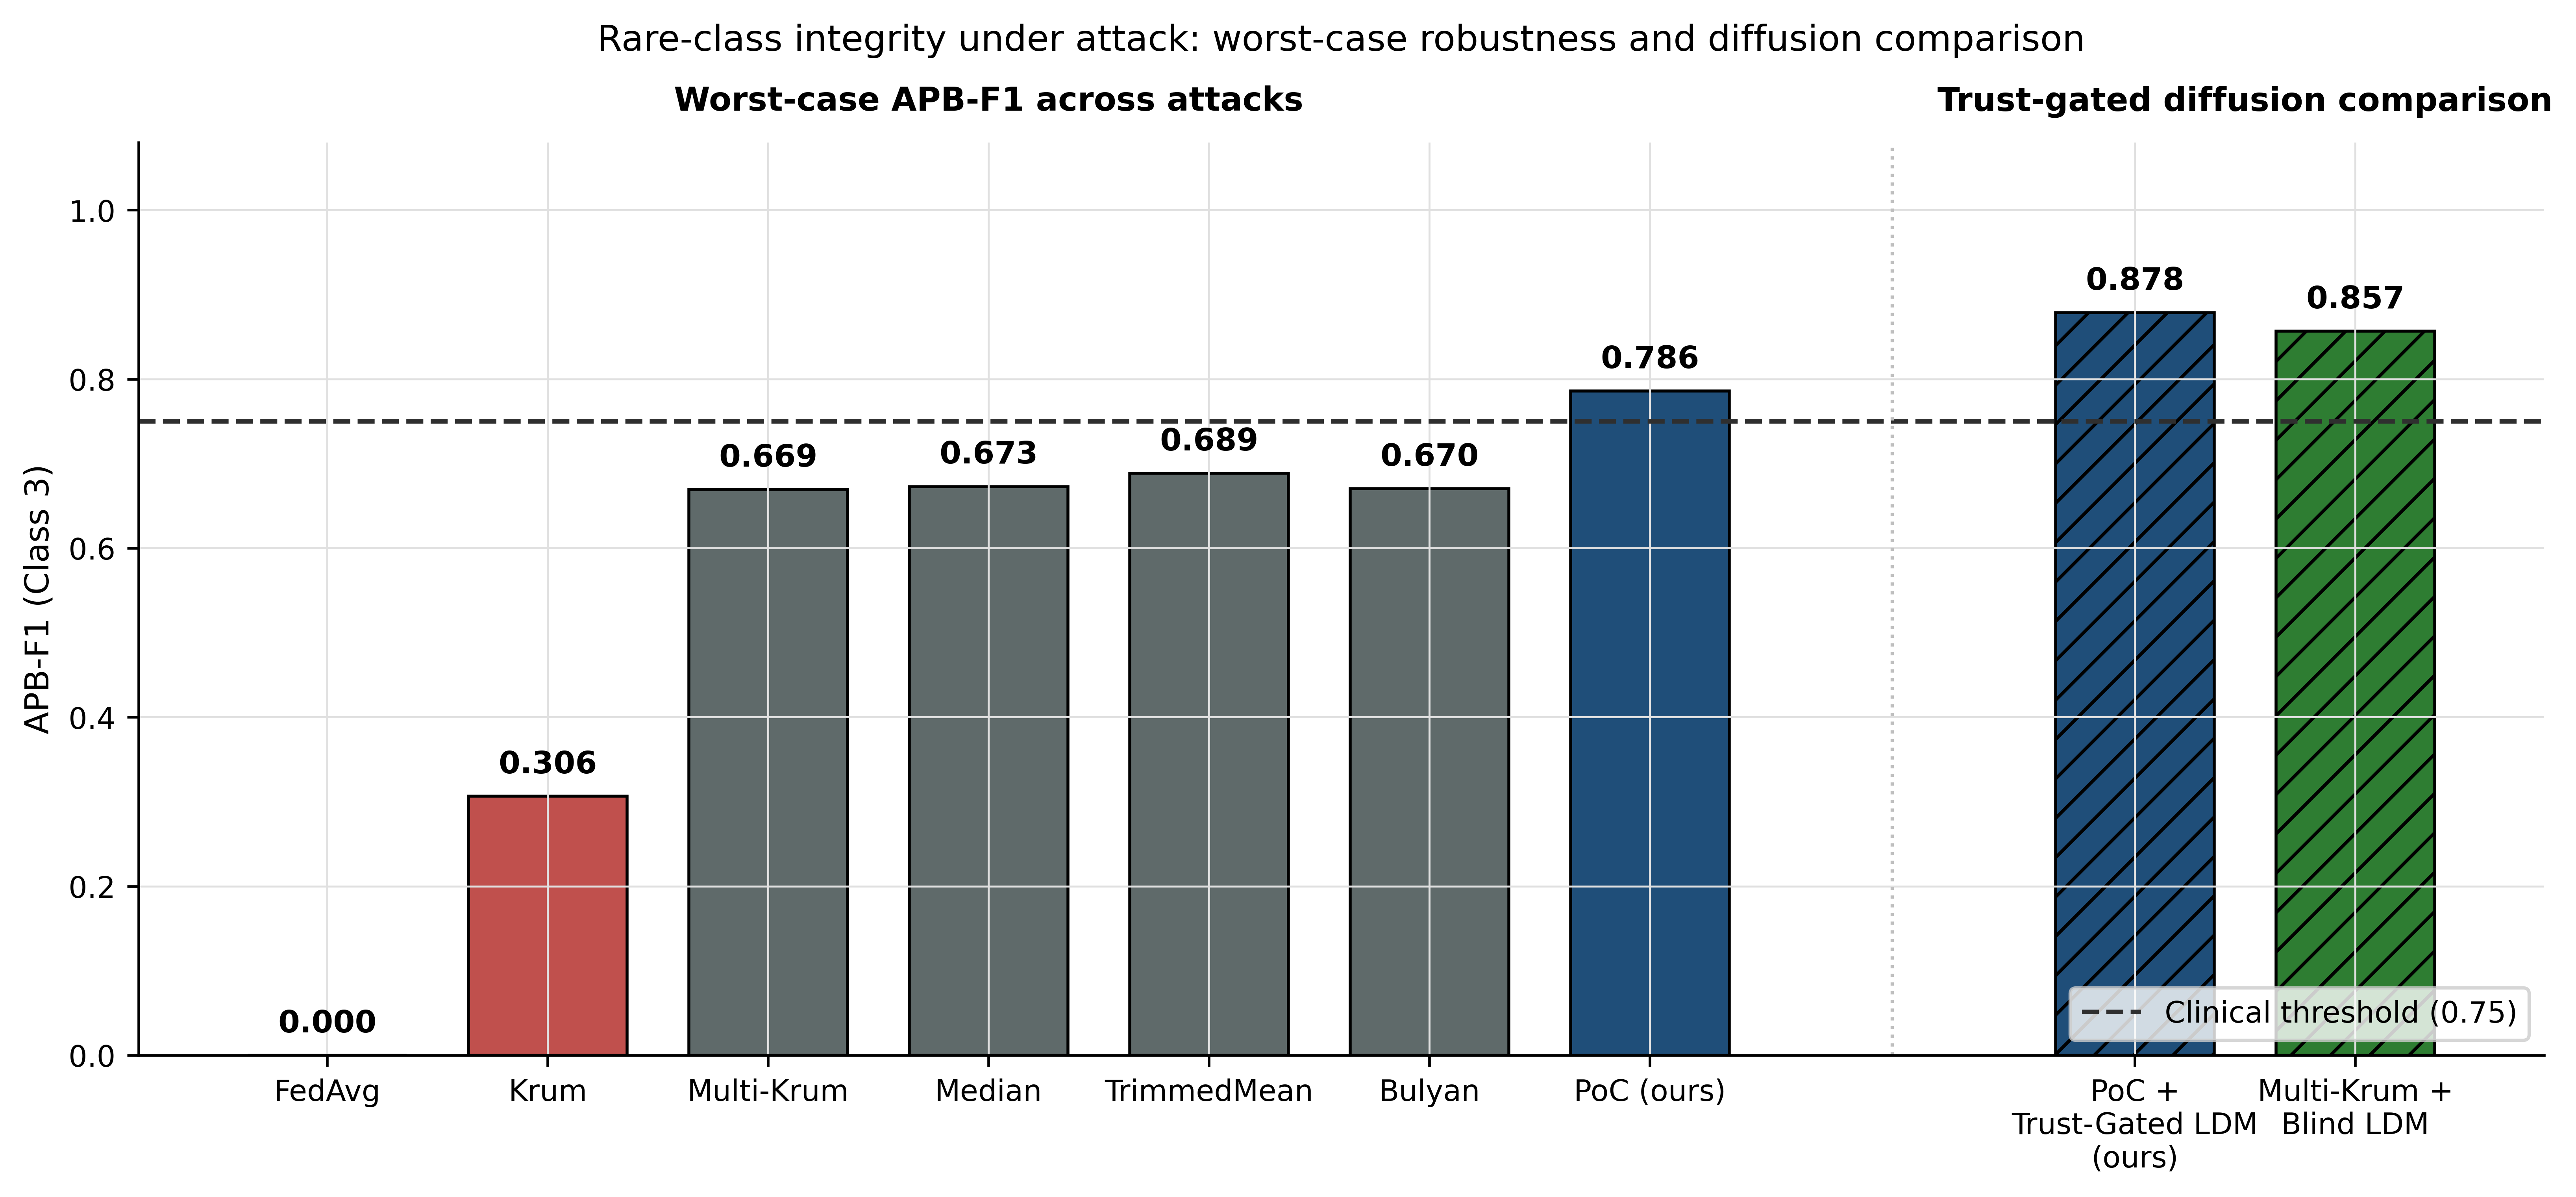
\includegraphics[width=\linewidth]{figures_phase3/fig_apb_with_ldm.png}
\caption{Rare-class integrity under attack. Left: worst-case APB-F1
across the three attacks per defence. Right: final-round APB-F1
under the two diffusion-augmented policies under the sleeper attack.
The dashed line is the $0.75$ clinical threshold.}
\label{fig:synthesis}
\end{figure}

On the left, \fedavg has worst-case APB-F1 $=0.000$ (from Gaussian),
\krum $=0.306$ (from sleeper), the four distance-based aggregators
cluster between $0.67$ and $0.69$, and \poc alone sits above $0.75$
at $0.786$. On the right, adding trust-gated diffusion on top of
\poc raises APB-F1 to $0.879$, and adding blind diffusion on top of
\mkrum raises it to $0.857$. On APB-F1 alone the two cells are
close; but Fig.~\ref{fig:bsr} showed that the blind-diffusion gain
comes together with a higher final-round BSR. The ledger therefore
acts as a precision-increasing augmentation policy in the sleeper
regime: it keeps positive APB predictions trustworthy while
admitting essentially the same recall as the blind baseline.

% ============================================================================
\section{Discussion and Limitations}
\label{sec:discussion}

The sleeper attack is informative because it separates what two
classes of defences can observe. \krum sees only the current
round's weight vectors; \poc sees a history of each client's
validation accuracies. The sleeper is designed to hide in the
geometric signal, but it cannot hide in the behavioural one,
because flipping labels reduces the Byzantine client's own
validation accuracy on honest data. Any history-based score that
responds to this can see the attack, and the PoC score used here is
arguably the simplest such score.

The macro-F1 win for \fedavg under the stealthier attacks (see
Fig.~\ref{fig:macro_heatmap}) is not a safety claim for \fedavg. The
same algorithm collapses under Gaussian, and macro-F1 systematically
obscures the minority-class failure that matters clinically. The
gain from trust-gating over blind diffusion is small on APB-F1 (the
right block of Fig.~\ref{fig:synthesis} shows about two points), but
the more interesting effect lives in Fig.~\ref{fig:bsr}: the blind
baseline keeps admitting attacker requests, so its BSR drifts
upward at the end of training, while the PoC gate shuts that channel
off once the behavioural score has caught up. A positive APB
prediction coming out of \actledger is therefore more trustworthy
than one coming out of the blind baseline, even when both have the
same APB-F1.

It is worth being explicit about what the ledger is, because this
is where the blockchain-FL literature has a history of over-claiming.
PoC is an on-chain, history-based contribution score; it is not a
cryptographic proof and \actledger is not a consensus protocol. The
ledger has exactly two concrete roles: it persists the update,
round-completion, and synthetic-pipeline events with tamper-evident
semantics (so that post-hoc forensic reconstruction is possible),
and it exposes the behavioural history on which PoC is computed.
Neither role requires a novel consensus design.

Each grid cell is reported from a single-seed execution. Running
forty communication rounds of FL alongside synchronous inference of
a latent-diffusion generator is compute-heavy, and a full multi-seed
variance map sat outside the available budget for this proof of
concept; the stark separation between un-gated and gated aggregation
under the sleeper attack is nonetheless a structural effect that is
expected to reproduce under replication. A detailed systems
accounting of on-chain gas costs is also out of scope here; the
focus is the algorithmic security of the trust-gated diffusion
pipeline and the auditability of the event log rather than any claim
about the economics of the ledger. The attacker ratio is fixed at
twenty percent throughout, and Fang et al.~\cite{fang2020local}
showed that higher ratios can compromise both geometric and
behavioural rules in different ways. The attack set evaluated here
does not cover the variant of the augmentation bypass in which the
attacker trains its own generator and shares only samples rather
than requests; the same gate is expected to handle it but this has
not been tested. Finally, cross-dataset generalisation (for example
to 12-lead records or PTB-XL~\cite{jimenez2024ecg}) is not reported;
that is a straightforward follow-up.

% ============================================================================
\section{Conclusion}
\label{sec:conclusion}

This paper presented \actledger, a blockchain-orchestrated FL
system for clinical ECG classification that couples a behavioural,
history-based contribution score with a trust-gated
class-conditional latent diffusion generator. Under three
qualitatively different attacks on aggregation, \poc is the only
defence among seven that keeps APB-F1 above the $0.75$ deployability
line. Adding trust-gated diffusion further raises APB-F1 to
$0.879$ under the sleeper attack while lowering the final-round
backdoor success rate compared with an un-gated baseline. The
contribution to the security community is the observation that the augmentation pipeline is
a separate attack surface, that closing it requires a behavioural
signal which geometric aggregation cannot provide, and that an
append-only event log makes every aggregation and augmentation
decision individually auditable without any cryptographic-proof
machinery.

% ============================================================================
\begin{thebibliography}{99}

\bibitem{mcmahan2017fedavg}
McMahan, B., Moore, E., Ramage, D., Hampson, S., Arcas, B.A.y.:
Communication-Efficient Learning of Deep Networks from Decentralized
Data. In: Proc. 20th Int.\ Conf.\ on Artificial Intelligence and
Statistics (AISTATS), PMLR vol.~54, pp.~1273--1282 (2017).

\bibitem{kairouz2021advances}
Kairouz, P., McMahan, H.B., Avent, B., et al.: Advances and Open
Problems in Federated Learning. Foundations and Trends in Machine
Learning \textbf{14}(1--2), 1--210 (2021). \doi{10.1561/2200000083}

\bibitem{moody2001mitbih}
Moody, G.B., Mark, R.G.: The Impact of the MIT-BIH Arrhythmia
Database. IEEE Engineering in Medicine and Biology Magazine
\textbf{20}(3), 45--50 (2001). \doi{10.1109/51.932724}

\bibitem{aami1998ec57}
Association for the Advancement of Medical Instrumentation:
ANSI/AAMI EC57:1998/(R)2003 -- Testing and Reporting Performance
Results of Cardiac Rhythm and ST-Segment Measurement Algorithms.
AAMI, Arlington, VA (1998; reaffirmed 2003 and 2008).

\bibitem{blanchard2017krum}
Blanchard, P., El Mhamdi, E.M., Guerraoui, R., Stainer, J.:
Machine Learning with Adversaries: Byzantine Tolerant Gradient
Descent. In: Advances in Neural Information Processing Systems
(NeurIPS) (2017).

\bibitem{yin2018byzantine}
Yin, D., Chen, Y., Kannan, R., Bartlett, P.: Byzantine-Robust
Distributed Learning: Towards Optimal Statistical Rates. In:
Proc.\ 35th Int.\ Conf.\ on Machine Learning (ICML), PMLR
vol.~80, pp.~5650--5659 (2018).

\bibitem{elmhamdi2018bulyan}
El Mhamdi, E.M., Guerraoui, R., Rouault, S.: The Hidden
Vulnerability of Distributed Learning in Byzantium. In:
Proc.\ 35th Int.\ Conf.\ on Machine Learning (ICML), PMLR
vol.~80, pp.~3521--3530 (2018).

\bibitem{fang2020local}
Fang, M., Cao, X., Jia, J., Gong, N.Z.: Local Model Poisoning
Attacks to Byzantine-Robust Federated Learning. In: 29th USENIX
Security Symposium, pp.~1605--1622 (2020).

\bibitem{bagdasaryan2020how}
Bagdasaryan, E., Veit, A., Hua, Y., Estrin, D., Shmatikov, V.:
How To Backdoor Federated Learning. In: Proc.\ 23rd Int.\ Conf.\
on Artificial Intelligence and Statistics (AISTATS), PMLR
vol.~108, pp.~2938--2948 (2020).

\bibitem{zhuang2024bclayers}
Zhuang, H., Yu, M., Wang, H., Hua, Y., Li, J., Yuan, X.:
Backdoor Federated Learning by Poisoning Backdoor-Critical
Layers. In: Proc.\ Int.\ Conf.\ on Learning Representations
(ICLR) (2024). arXiv:2308.04466

\bibitem{foroughi2026lsa}
Foroughi, M.H., Rastegar, S.H., Sabokrou, M., Khonsari, A.:
Exploiting Layer-Specific Vulnerabilities to Backdoor Attack in
Federated Learning. arXiv:2602.15161 (2026). To appear in
IEEE International Conference on Communications (ICC) 2026.

\bibitem{ho2020ddpm}
Ho, J., Jain, A., Abbeel, P.: Denoising Diffusion Probabilistic
Models. In: Advances in Neural Information Processing Systems
(NeurIPS) (2020).

\bibitem{rombach2022ldm}
Rombach, R., Blattmann, A., Lorenz, D., Esser, P., Ommer, B.:
High-Resolution Image Synthesis with Latent Diffusion Models.
In: Proc.\ IEEE/CVF Conf.\ on Computer Vision and Pattern
Recognition (CVPR), pp.~10684--10695 (2022).

\bibitem{kim2020blockfl}
Kim, H., Park, J., Bennis, M., Kim, S.-L.: Blockchained
On-Device Federated Learning. IEEE Communications Letters
\textbf{24}(6), 1279--1283 (2020). \doi{10.1109/LCOMM.2019.2921755}

\bibitem{kang2019incentive}
Kang, J., Xiong, Z., Niyato, D., Xie, S., Zhang, J.: Incentive
Mechanism for Reliable Federated Learning: A Joint Optimization
Approach to Combining Reputation and Contract Theory. IEEE
Internet of Things Journal \textbf{6}(6), 10700--10714 (2019).
\doi{10.1109/JIOT.2019.2940820}

\bibitem{kang2020reliable}
Kang, J., Xiong, Z., Niyato, D., Zou, Y., Zhang, Y., Guizani, M.:
Reliable Federated Learning for Mobile Networks. IEEE Wireless
Communications \textbf{27}(2), 72--80 (2020).
\doi{10.1109/MWC.001.1900119}

\bibitem{li2021bcflsurvey}
Li, D., Han, D., Weng, T., Zheng, Z., Li, H., Liu, H., Castiglione,
A., Li, K.-C.: Blockchain for Federated Learning Toward Secure
Distributed Machine Learning Systems: A Systemic Survey. Soft
Computing (2021). \doi{10.1007/s00500-021-06496-5}

\bibitem{brisimi2018ehr}
Brisimi, T.S., Chen, R., Mela, T., Olshevsky, A., Paschalidis,
I.C., Shi, W.: Federated Learning of Predictive Models from
Federated Electronic Health Records. Int.\ J.\ Medical
Informatics \textbf{112}, 59--67 (2018).
\doi{10.1016/j.ijmedinf.2018.01.007}

\bibitem{jimenez2024ecg}
Jimenez Gutierrez, D.M., Hassan, H.M., Landi, L., Vitaletti, A.,
Chatzigiannakis, I.: Application of Federated Learning
Techniques for Arrhythmia Classification Using 12-Lead ECG
Signals. arXiv:2208.10993 (2024).

\end{thebibliography}

\end{document}
